%Se podrá presentar en dos Capítulos separados: Capítulo 4: Resultados y Capítulo 5: Discusión

%HIPÓTESIS: la linealidad se mantiene o no con la escala

\section {Bloque/Núcleo 1-A1-Propuesta de relevamiento por imágenes RGB de las reservas de la provincia de Misiones}
%Comenzaría por una descripción territorial de las reservas, proponiendo una clasificación, que puede ser por público o privada, ubicación, superficie, etc. Luego vendría una propuesta de las opciones: satelital, aérea tripulada y aérea no tripulada, restringiendonos a imágenes RGB. Acompaña a cada opción un análisis técnico económico. Finalmente, concluir con cuál sería la mejor opción dependiendo del tipo de reserva y la resolución pretendida. Brindar una herramienta de toma de decisión para quien desee hacer un relevamiento de reservas en la provincia de Misiones.
El propósito de esta sección es realizar un análisis comparativo del relevamiento entre distintas áreas de reservas forestales. Se consideran casos extremos en extensión grande como es la reserva Biósfera Yaboty, de más de 250 mil hectáreas, y por otro lado se analizan algunas reservas públicas o privadas de alrededor de pocas hectáreas de extensión. El objetivo es obtener herramientas que faciliten la toma de decisiones sobre la estrategia adecuada para el relevamiento y monitoreo forestal, tanto en el ámbito público como el privado, en la provincia de Misiones. Los parámetros que son considerados para el análisis son el tiempo que implica la captura de imágenes, la necesidad de recursos para almacenamiento, requerimientos económicos y restricciones legales y reglamentarias.
\subsection{Reservas de bosque nativo de la Selva Paranaense en la Provincia de Misiones}
El remanente en pie del bioma conocido como Bosque Atlántico o Selva Paranaense representa hoy un 5\% de la histórica extensión, que cubría desde toda la provincia de Misiones, buena parte del Paraguay y el sur de Brasil. En la provincia de Misiones está presente casi la mitad de ese remanente, existiendo varias reservas, tanto públicas como privadas. Algunas de ellas son descriptas en el presente trabajo.
\subsubsection{Reserva Biósfera Yaboty}
Para conocer de manera aproximada el tiempo que sería necesario para completar un relevamiento fotográfico aéreo territorial, tomamos como ejemplo el área de la biosfera Yaboty, cuya extensión es de 253.773 ha [1].
\begin{table}[H]
    \centering
    \begin{tabular}{|c|c|c|}
        \hline
        \textbf{Reserva} & Biósfera Yaboty &   \multirow{ 3}{*}{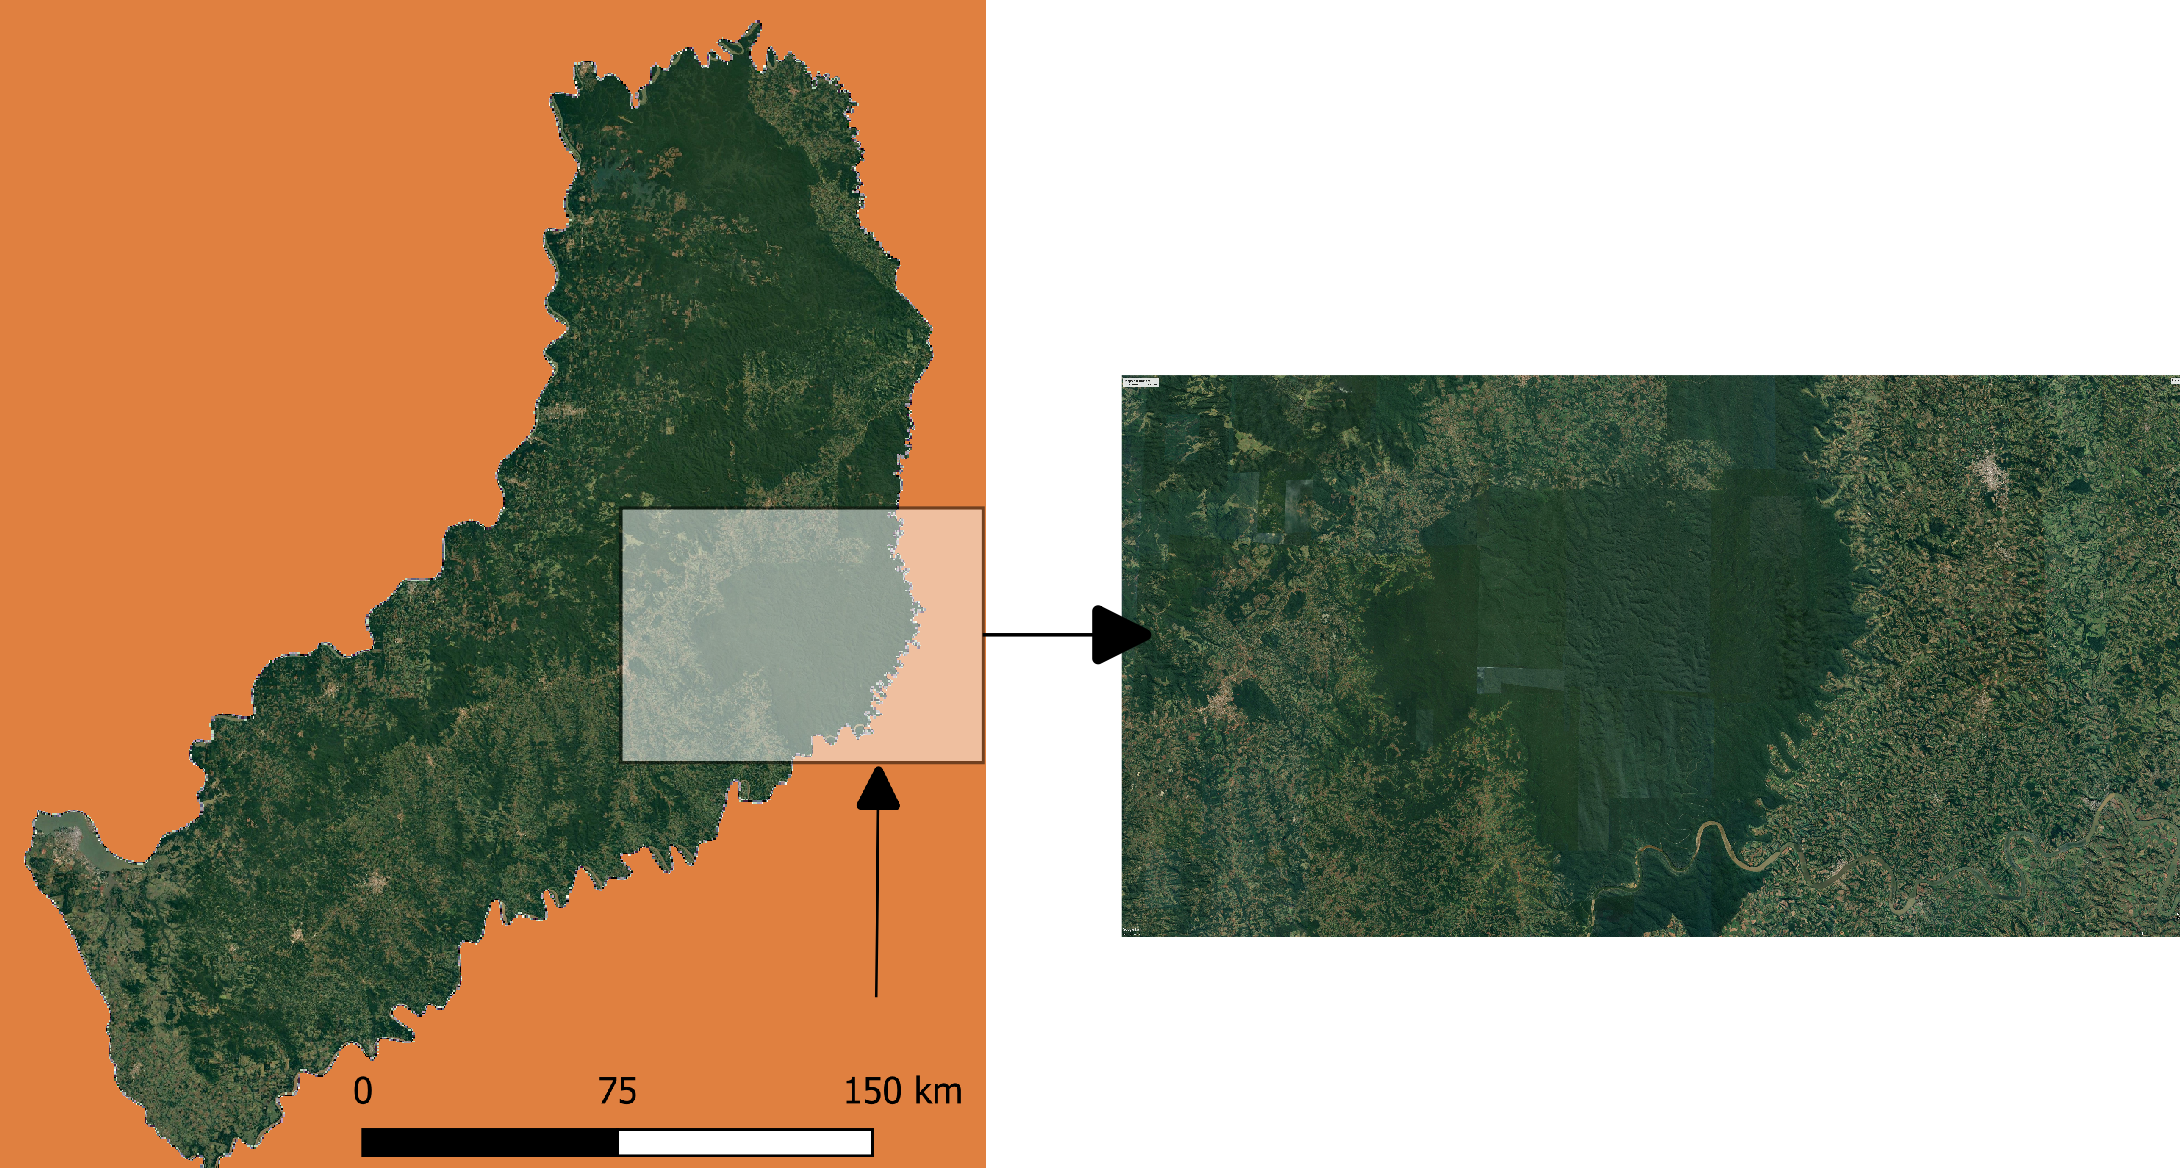
\includegraphics[width=30mm]{Imagenes/Yaboty.png}}\\ 
        \textbf{Administración} & Pública\\
        \textbf{Ubicación} & E 53° 40’, O 54° 18’, N 26° 37’ S 27° 12’ \\
        \textbf{Superficie} & 253.773 ha\\
        \hline
    \end{tabular}
    \label{Yaboty}
\end{table}
\subsubsection{Reserva San Sebastián de la Selva}
\begin{table}[H]
\centering
\begin{tabular}{|c|c|c|}
\hline
 \textbf{Reserva} & San Sebastián de la Selva &   \multirow{ 3}{*}{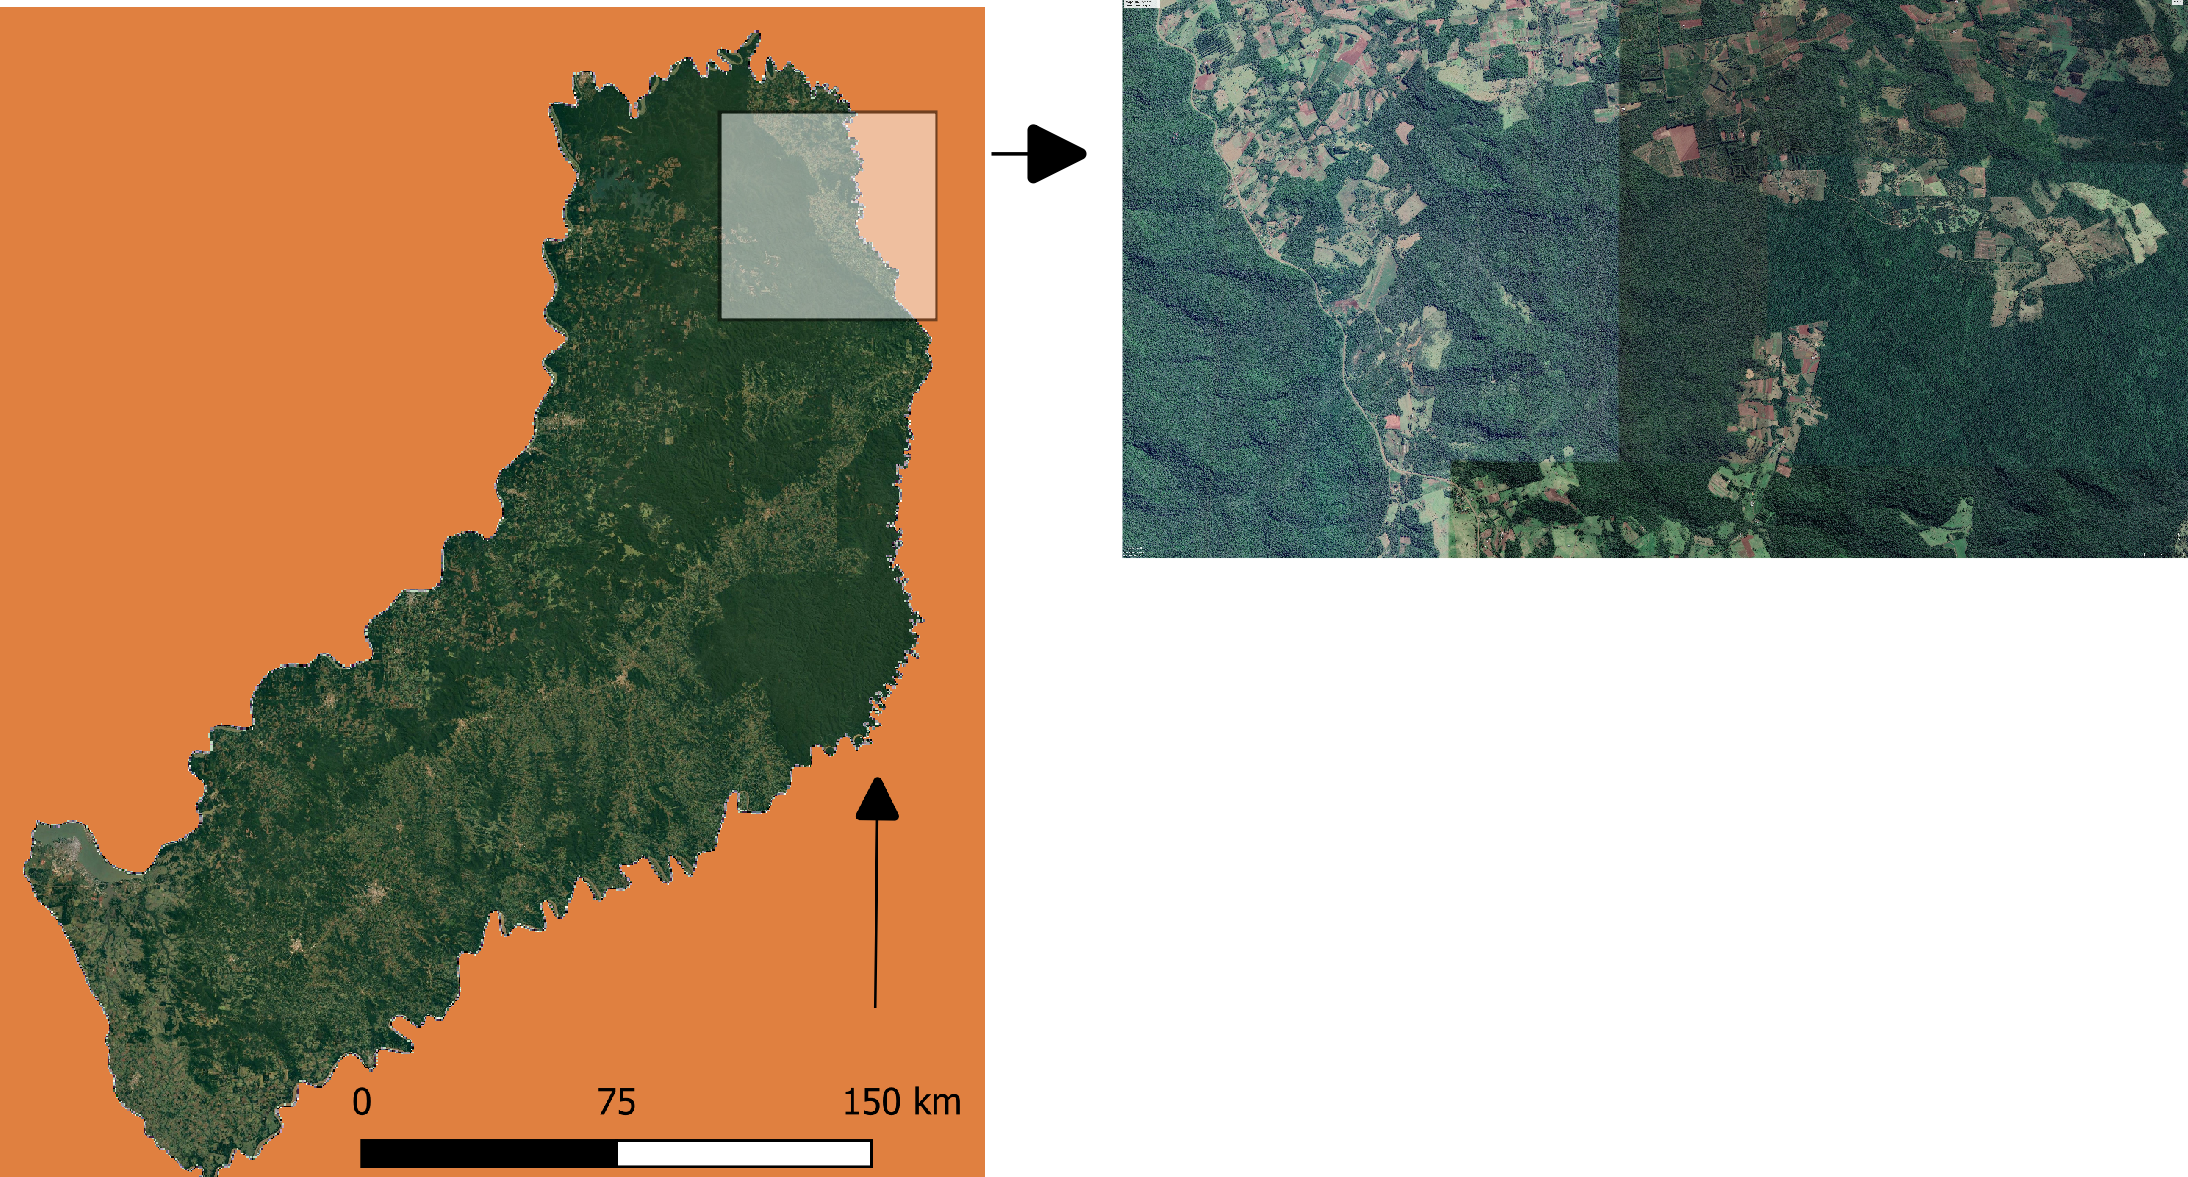
\includegraphics[width=30mm]{Imagenes/San Sebastian.png}}\\ 
\textbf{Administración} & Privada\\
        
        \textbf{Ubicación} & -25.857, -53.976 \\
         
        \textbf{Superficie} & 92 ha\\
\hline        
\end{tabular}

\label{Profundidad}
\end{table}
La reserva San Sebastián de la Selva es una reserva privada de cien hectáreas, que contiene áreas de selva virgen y de selva en restauración. Está ubicada en la localidad de Comandante Andresito, al norte de la provincia de Misiones, sobre la ruta nacional 101, entre los parques Urugua-í y Foerster. 
\subsubsection{Parque Provincial Cañadón de Profundidad}
\begin{table}[H]
\centering
\begin{tabular}{|c|c|c|}
\hline
 \textbf{Reserva} & Parque Provincial Cañadón de Profundidad &   \multirow{ 3}{*}{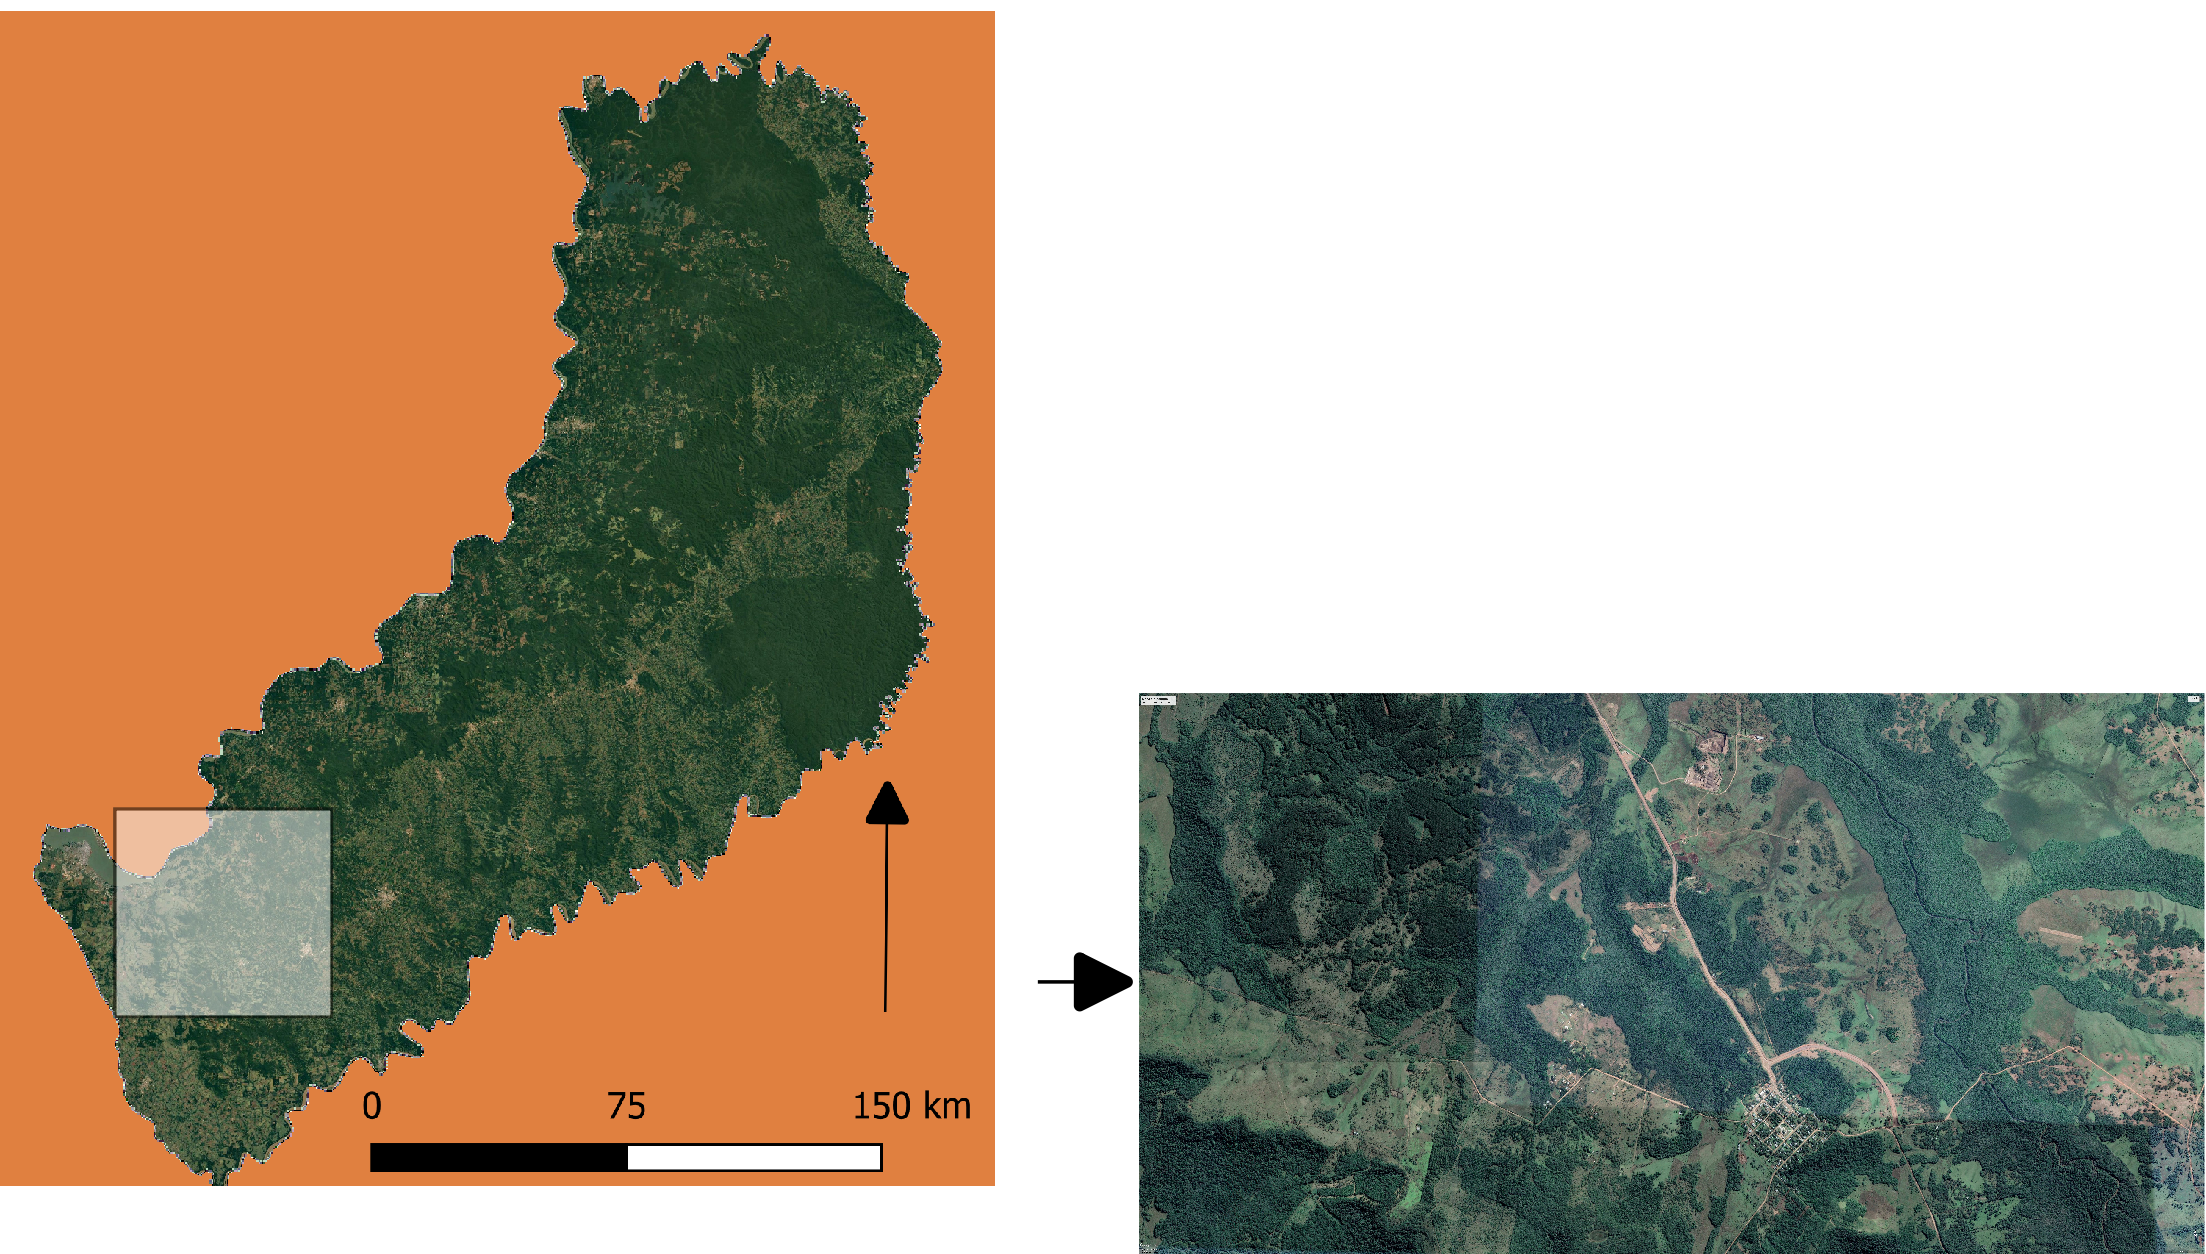
\includegraphics[width=30mm]{Imagenes/Profundidad.png}}\\ 
\textbf{Administración} & Pública\\
        
        \textbf{Ubicación} & -27.558, -55.702 \\
         
        \textbf{Superficie} & 19 ha\\
\hline        
\end{tabular}

\label{Profundidad}
\end{table}
\subsection{Plataformas para el sensado remoto}
En este apartado se analizarán las principales características de las opciones de plataformas para el sensado remoto. El análisis se limitará a la opción de uso de sensores de espectro visible.
\subsubsection{Imaginería satelital}
Se entiende por satélite artificial a todo dispositivo fabricado por el humano que es puesto en órbita alrededor del planeta Tierra con diversos propósitos que abarcan desde el establecimiento de comunicaciones hasta la observación terrestre por medio del sensado remoto. Éste último es el que reviste interés para el presente trabajo. Los satélites para sensado remoto van generalmente equipados con sensores multiespectrales, con múltiples bandas. La operación de los satélites es de manera continua desde que son puestos en órbita hasta el fin de su vida útil, varios años después. El lanzamiento y puesta en órbita requiere de infraestructura adecuada a tal fin, de las cuales hay muy pocas en el mundo, concentradas en no más de una decena de países. Los datos recopilados por los satélites son transmitidos a estaciones terrenas ubicadas en distintos puntos del planeta, y el acceso a las imágenes de alta resolución suele ser restringido a una contraprestación monetaria. No obstante suele haber acceso gratuito a imágenes con menor resolución. Las imágenes satelitales se definen por sus características de resolución, que son cuatro: resolución espacial, espectral, temporal y radiométrica.

Según la base de datos de la Unión de Científicos Conscientes \cite{noauthor_satellite_nodate}, actualizada el primero de mayo de 2.022, existen alrededor de 5.500 satélites orbitando la Tierra, de los cuales 1.156 (es decir un 21\%)tienen por finalidad la observación terrestre. Son utilizados varios tipos de sensores considerando el rango de frecuencias o la longitud de onda para cuya adquisición han sido diseñados. Se destacan los de luz visible, infrarrojo cercano (near infrared - NIR), infrarrojo térmico (thermal infrared - TIR), pancromático e infrarrojo de onda corta (shortwave infrared - SWIR). También existe un considerable despliegue de radares de apertura sintética (synthetic aperture radar - SAR) en diferentes bandas. De los satélites de observación terrestre, aproximadamente un 40\% son con sensores ópticos, es decir, capturan imágenes en el espectro visible.
Hay muchas y muy diversas fuentes de imágenes satelitales, tanto en forma gratuita como pagas. Entre las opciones pagas, imágenes multiespectracles con una resolución espacial de 50 cm se consiguen por montos entre 10 dólares por km\textsuperscript{2} hasta 29 dólares por km\textsuperscript{2} según sean actualizadas o de archivo (más de 90 días)\cite{noauthor_satellite_2020}. Debe tenerse en cuenta el tamaño mínimo del área a ser adquirida, en caso de las imágenes de archivo son 25 km\textsuperscript{2} (2500 ha) y las actualizadas son de 100 km\textsuperscript{2} (10000 ha).
\begin{table}[H]
    \centering
    \caption{Características de sensores satelitales. Fuente \cite{noauthor_3_nodate}}
    \begin{tabular}{|c|p{20mm}|p{15mm}|p{15mm}|p{25mm}|p{20mm}|p{20mm}|p{20mm}|}
        \hline
        \textbf{Sensor} & \textbf{Tamaño de imagen} & \multicolumn{4}{c}{\textbf{Resolución}} & \textbf{Aplicación principal} \\
        %\hline
        & & \textbf{Espacial} & \textbf{Temporal} & \textbf{Radiométrica} & \textbf{Espectral}  &\\
        \hline \hline
        Meteosat & Toda la esfera & 	2500 m 	& 0.5 h 	& 256 ND 	& 1Vis 1IR 1 IT & Meteorología\\
        \hline
        NOAA AVHRR & 2700 x 2700 km	& 1100 m 	 	& 12 h 	& 1024 ND 	& 2Vis 1IR 1IT & Observación atmosférica\\
        \hline
        Landsat TM 	& 185 x 185 km & 30 m 	 	& 16 d 	& 256 ND 	& 3Vis 3IR 1IT & Observación terrestre\\
        \hline
        SPOT HRV & 60 x 60 km	& 20 m 	 	& 20 d	& 256 ND 	& 2Vis 1IR & Observación terrestre\\
        \hline
        SPOT Vegetation & 2200 x 200 km	& 1150 m 	 	& 1 d	& 1024 ND 	& 2Vis 2IR & Monitoreo agrícola\\
        \hline
        MODIS & 2330 x 2330 km	& 250 - 100 m 	 km 	& 1 d	& 1024 ND 	& 36 bandas & Observación terrestre\\
        \hline
        IKONOS & 100 x 100 km	& 4 m 	 	& 3 d 	& 2048 ND 	& 3Vis 1IR & Observación terrestre\\
        \hline
        Albedo & 35 x 7 km & 0,4 m  & 1 d & S/D & 3Vis 1IR & Observación terrestre\\
        \hline
         Worldview & 13 x 13 km &   & 1 d & 2048 & 29 bandas & Observación terrestre\\
        \hline
         Sentinel & 13 x 13 km &  10 m & 1 d & S/D & 13 bandas & Observación terrestre\\
        \hline
    \end{tabular}

\label{Satelites}
\end{table}
\subsubsection{Aeronaves convencionales tripuladas}
Aquí se agrupan las aeronaves de determinado porte, cuya operación debe hacerse con tripulación, requiriendo que sea personal capacitado y con licencia para operarlos. En esta categoría se incluyen los aviones de ala fija, como los de ala rotatoria (helicópteros) así como aerostatos. Su operación requiere de una planificación de vuelo que debe ser reportada al área de espacio de vuelo controlado, además de necesitar una base de despegue y aterrizaje. El marco regulatorio de estas operaciones son las Regulaciones Argentinas de la Aviación Civil (RAAC), Parte 91 \cite{noauthor_infoleg_nodate-1}.
\paragraph{Cámaras fotográficas}
Algunos tipos de cámaras utilizadas a bordo de aeronaves tripuladas para realizar relevamientos fotogramétricos:
Vexcel UltraCam Eagle

%Se podría añadir como figura un mapa con las regiones de información de vuelo (FIR), con las zonas de control, aeródromos habilitados, por ejemplo, etc.
\subsubsection{Aeronaves no tripuladas}
Generalmente conocidos como VANT, los vehículos aéreos no tripulados (VANT) son cada vez más asequibles por el público general. Disponibles en amplia variedad de modelos, constituyen una formidable herramienta para llevar a cabo tareas de relevamiento aéreo. El abanico de posibilidades se ve ampliado por la prescindencia de una pista de despegue o aterrizaje de dimensiones grandes. El marco legal regulatorio para la actividad con VANT es la resolución ANAC 885 \cite{noauthor_infoleg_nodate}.
Existe una amplia variedad de tipos de VANT, que pueden ser de múltiples rotores o de ala fija. El propósito del presente trabajo no es exhaustivo en este aspecto, pero a los efectos de describir las características principales, se lo hará con algunos de ellos.
\paragraph{Multirrotor}
Los VANT tipo multirrotor poseen cuatro o más hélices para proporcionar al vehículo la sustentación y la propulsión en tres ejes de desplazamiento. Esta característica es la que le confiere mayor maniobrabilidad, especialmente en espacios reducidos. La energía para propulsarse es eléctrica, proveniente de baterías. Son los más difundidos comercialmente.
\subparagraph{DJI Mini 2}
Un dron comercial asequible es el Mini 2 del fabricante DJI \cite{noauthor_dji_nodate-1}. Está equipado con una cámara con sensor 1/2.3” CMOS, de 12 millones de píxeles efectivos. La lente de la cámara posee un ángulo de visión de 83º y un formato equivalente a 35 mm de longitud focal de 24 mm, una apertura de f/2.8 y un rango focal de 1 m hasta infinito. En cuanto a las velocidades, el dron tiene tres modos de funcionamiento, modo Sport, modo Normal y modo Cine. En Sport se desplaza hasta 16 m/s, en modo normal 10 m/s y en modo cine 6 m/s.
\subparagraph{DJI Mavic 3M}
Este es un dron profesional \cite{noauthor_dji_nodate}. Cuenta con una cámara RGB de 4/3 CMOS, con 20 millones de píxeles efectivos. La lente es de un campo de visión de 84º, con una longitud focal equivalente de 24 mm. La apertura es de f/2.8 a f/11, y foco de 1 m al infinito. En modo normal puede desplazarse hasta 15 m/s
\paragraph{Ala fija}
Este tipo de VANT poseen un ala fija que le brinda sustentación, por lo que pueden incluso planear aunque falle la planta motriz de la aeronave. Sus características de funcionamiento permiten vuelos más extensos, cubriendo mayores áreas. Existen VANT de ala fija alimentados eléctricamente con baterías o con motores de combustión interna. Se los encuentra esencialmente en aplicaciones de agricultura de precisión y en el campo militar. 
\subparagraph{Asesor/9}
Es un VANT de ala fija de casi 2 m de envergadura \cite{noauthor_drone_nodate}. Puede desplazarse a 17 m/s y tiene una autonomía de dos horas de vuelo. Va equipado con una cámara multiespectral MicaSense Altum-PT \cite{noauthor_altum-pt_2023} cuyo sensor es de 12,4 millones de píxeles, que le confieren una resolución de 5,28 cm/pixel volando a 120 m sobre el terreno.

Sensor
12.4 MP sensor pancromático
Cinco bandas espectrales de 3.2 MP
Resolución
Multiespectral (pan-sharpened): 1.24cm/pixel a 60m; 2.49cm/pixel a 120m

RGB12.4 MP (obturador global, alineado con todas las bandas)
Sensor térmicoFLIR LWIR infrarrojo térmico 7.5-13.5um calibrado radiométricamente
RESOLUCIÓN5.28 cm cm / pixel (por banda MS), 33.5 cm / pixel (banda térmica), 2.49 cm / pixel (pancro) a 120 m AGL
VELOCIDAD DE CAPTURAHasta 3 capturas por segundo DNG sin procesar
INTERFACES3 GPIO: señal de disparo, salida de la parte superior del cuadro, salida de 1 PPS, botón host. Puerto USB 2.0 para WiFi, ethernet 10/100/1000, serial, y almacenamiento CFexpress
CAMPO DE VISIÓN50° HFOV x 38° VFOV (MS) / 44° HFOV x 38° VFOV (PAN)
\subsection{Requerimientos y restricciones}
Para llevar adelante el relevamiento de las áreas forestales hay que tener en cuenta los requerimientos en el tiempo y en el equipamiento, así como las restricciones que imponen las regulaciones legales y condiciones geográficas y meteorológicas. Dependiendo de cuán grande sea el área a relevar, puede resultar más conveniente alguna de las plataformas de sensado remoto que otra. El criterio que debe ponderarse está basado en cálculos de tiempo, de costos operacionales y de disponibilidad. Para distintos escenarios, reservas grandes de miles de hectáreas de extensión o pequeñas reservas privadas de pocas decenas o centenas de hectáreas, los cálculos arrojarán resultados diferentes.
\subsubsection{Cálculo de factor de escala}
Los sensores remotos que serán tratados en el presente trabajo son del tipo pasivo, es decir, están compuestos por detectores que registran las ondas de luz solar reflejadas en el terreno. Particularmente nos interesan los que cubren el espectro visible. Básicamente constituyen una cámara fotográfica, que se compone de un arreglo de lentes y espejos que refractan y reflejan la luz, proyectándola sobre un sensor fotosensible, generalmente es un rectángulo conformado como un arreglo de detectores, cada uno de ellos representa a un pixel de la imagen. Según las características de estos sensores y la configuración de lentes, la distancia al objetivo, la resolución espacial queda determinada. 
Para poder comparar entre las diferentes opciones de plataformas para captura de imágenes aeroespaciales, es necesario conocer determinados parámetros de cada una. Un parámetro es el tiempo necesario para captura de imágenes de un determinado área. El costo asociado a la operación de captura de imágenes es otro parámetro a ser tenido en cuenta. Finalmente hay otros parámetros sobre los que las opciones pueden soportarse. Uno es el porcentaje de área útil sobre área total relevada. Otro parámetro es el espacio de almacenamiento requerido.
Si se comparan imágenes obtenidas por satélites contra aquellas obtenidas por aeronaves tripuladas o VANT, resulta evidente que aquellas cubren una extensión mayor, por lo que una sola captura puede exceder en mucho la zona de interés. En el caso de las imágenes aéreas es muy probable que sean necesarias varias imágenes para cubrir la zona de interés. Si se pretende construir un ortomosaico con esas imágenes, es necesario garantizar al momento de realizar las capturas un mínimo nivel de solapamiento entre capturas consecutivas (60\%) y entre aquellas que pertenecen a líneas de vuelo adyacentes (25\%). Los satélites son básicamente cámaras que orbitan alrededor del planeta que capturan imágenes de manera regular, continua, las cuales se  almacenan temporalmente en el satélite y son descargadas a estaciones de enlace para luego ser comercializadas. De modo que a requerimiento, las imágenes suelen estar disponibles. diferente es el caso de las imágenes aéreas, para las cuales se define un vuelo específico- Eso conlleva otros tiempos, ya que implica programar y preparar el vuelo, eventualmente trasladar la aeronave si es tripulada desde el aeródromo del cual despega y al cual regresa para aterrizar, y la duración misma del procedimiento de captura. Entre las variables que intervienen en la duración del vuelo en la fase de captura de imágenes se puede mencionar la de la extensión del área de interés, la velocidad de desplazamiento, la altura de vuelo. Esto también tendrá incidencia en la resolución espacial de las imágenes y en el espacio de almacenamiento requerido. Finalmente en el costo total del procedimiento, en el caso de aeronaves tripuladas incidirá el tiempo que lleve desde la puesta en marcha del motor hasta su apagado, ya que todo eso se contempla como hora de vuelo.
Los sensores, esto es, las cámaras que son llevadas como carga útil por las diferentes plataformas, están definidos por sus características. La distancia focal es un atributo de cada cámara. El factor de escala está dado por la altura de vuelo sobre el terreno, que puede variar incluso durante el vuelo, y por la distancia focal de la cámara, que es fija. 
\begin{figure}
    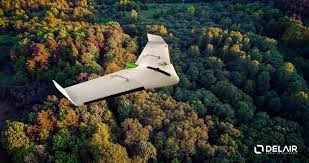
\includegraphics[width=\textwidth]{Imagenes/dron.jpg}
     \hfill
     \caption{Superposition of manual and automatic shadow masks (red contour and blue colored area), using 60th percentile, using ψ\textsubscript{BR} (blue an red channels) for the Invariant color index}
    \label{dron}
\end{figure}
Para hallar el factor de escala $m_b$, relacionamos la altura de vuelo $H_g$ con la distancia focal
de la cámara $f$ mediante la ecuación \ref{escala} \cite{linder_digital_2016}:
 %%%%%%%%%%%%%%%%%%%%%%%%%%%%%%%%%%%%%% ECUACIÓN %%%%%%%%%%%%%%%%%%%%%%%%%%%%%%%%%%%%%%%%%%%%%%%%%%%%%%%%%
\\
\begin{equation}
	m_b=\frac{H_g}{f},\label{escala}
\end{equation}
\\
%%%%%%%%%%%%%%%%%%%%%%%%%%%%%%%%%%%%%%%%%%%%%%%%%%%%%%%%%%%%%%%%%%%%%%%%%%%%%%%%%%%%%%%%%%%%%%%%%%%%%%%%%
Para hallar cualquier distancia en la superficie real a partir de la fotografía, se aplica la relación de escala:
 %%%%%%%%%%%%%%%%%%%%%%%%%%%%%%%%%%%%%% ECUACIÓN %%%%%%%%%%%%%%%%%%%%%%%%%%%%%%%%%%%%%%%%%%%%%%%%%%%%%%%%%
\\
\begin{equation}
	S=\frac{S'H_g}{f},\label{escala1}
\end{equation}
\\
%%%%%%%%%%%%%%%%%%%%%%%%%%%%%%%%%%%%%%%%%%%%%%%%%%%%%%%%%%%%%%%%%%%%%%%%%%%%%%%%%%%%%%%%%%%%%%%%%%%%%%%%%
donde $S$ es la distancia en la superficie real, $S'$ es la distancia en la imagen.
En un relevamiento fotogramétrico, el solapamiento longitudinal suele ser de un promedio de 60\%, mientras que el solapamiento lateral suele ser de 25\% [4]. La distancia longitudinal $B$ entre dos fotografías consecutivas (línea de base) se halla en función al solapamiento longitudinal $p$, y se calcula según la ecuación (\ref{linea_de_base}).
 %%%%%%%%%%%%%%%%%%%%%%%%%%%%%%%%%%%%%% ECUACIÓN %%%%%%%%%%%%%%%%%%%%%%%%%%%%%%%%%%%%%%%%%%%%%%%%%%%%%%%%%
\\
\begin{equation}
	B=S(1-\frac{p}{100}),\label{linea_de_base}
\end{equation}
\\
%%%%%%%%%%%%%%%%%%%%%%%%%%%%%%%%%%%%%%%%%%%%%%%%%%%%%%%%%%%%%%%%%%%%%%%%%%%%%%%%%%%%%%%%%%%%%%%%%%%%%%%%%
La distancia $a$ entre dos líneas de sobrevuelo adyacentes se define por el solapamiento lateral $q$.
  %%%%%%%%%%%%%%%%%%%%%%%%%%%%%%%%%%%%%% ECUACIÓN %%%%%%%%%%%%%%%%%%%%%%%%%%%%%%%%%%%%%%%%%%%%%%%%%%%%%%%%%
\\
\begin{equation}
	a=S(1-\frac{q}{100}),\label{distancia_adyacente}
\end{equation}
\\
%%%%%%%%%%%%%%%%%%%%%%%%%%%%%%%%%%%%%%%%%%%%%%%%%%%%%%%%%%%%%%%%%%%%%%%%%%%%%%%%%%%%%%%%%%%%%%%%%%%%%%%%%
Cuando se trata de un vuelo para realizar fotografías aéreas, ya sea tripulado o no, partiendo de conocer el área de interés, sus dimensiones, es posible definir las trayectorias de vuelo. De esta forma el relevamiento fotográfico aéreo se asemeja a una especie de "barrido", con varias líneas adyacentes. A lo largo de una línea se capturan imágenes de modo que se superpongan como mínimo en un 80\% dos fotografías consecutivas. Al final de cada línea la aeronave ejecuta un giro de 180º respecto al eje nadir-cenit de modo que al finalizar el giro su proa apunte en dirección contraria a la que tenía antes de iniciar el giro. Así inicia el recorrido de una nueva línea de vuelo, la cual es paralela a la anterior, separada una distancia que garantice un solapamiento mínimo de 25\%de imágenes en líneas de vuelo adyacentes. A partir de todo ello puede establecerse la cuenta de imágenes totales que cubran toda el área, así como el tiempo necesario para llevarlo a cabo. De esto también se obtiene el espacio de almacenamiento en memoria requerido.
La cantidad de imágenes por línea de vuelo $I_lv$ se puede conocer dada la longitud de la línea de vuelo $L_v$ y la línea de base $B$, mediante la ecuación (\ref{cantidad_imagenes}):
  %%%%%%%%%%%%%%%%%%%%%%%%%%%%%%%%%%%%%% ECUACIÓN %%%%%%%%%%%%%%%%%%%%%%%%%%%%%%%%%%%%%%%%%%%%%%%%%%%%%%%%%
\\
\begin{equation}
	I_{lv}=\frac{L_v}{B},\label{cantidad_imagenes}
\end{equation}
\\
%%%%%%%%%%%%%%%%%%%%%%%%%%%%%%%%%%%%%%%%%%%%%%%%%%%%%%%%%%%%%%%%%%%%%%%%%%%%%%%%%%%%%%%%%%%%%%%%%%%%%%%%%
Multiplicando el resultado de la ecuación \ref{cantidad_imagenes} por la cantidad de líneas de vuelo $N_{lv}$ se obtiene la cantidad total de imágenes $I_t$ para toda el área relevada:
  %%%%%%%%%%%%%%%%%%%%%%%%%%%%%%%%%%%%%% ECUACIÓN %%%%%%%%%%%%%%%%%%%%%%%%%%%%%%%%%%%%%%%%%%%%%%%%%%%%%%%%%
\\
\begin{equation}
	I_t={I_{lv}}{N_{Lv}},\label{cantidad_total_imagenes}
\end{equation}
\\
%%%%%%%%%%%%%%%%%%%%%%%%%%%%%%%%%%%%%%%%%%%%%%%%%%%%%%%%%%%%%%%%%%%%%%%%%%%%%%%%%%%%%%%%%%%%%%%%%%%%%%%%%
El espacio de almacenamiento necesario de cada imagen $M_i$ está determinado por las características de los sensores, la cantidad de píxeles $Px$, cantidad de bandas espectrales $B_e$, la profundidad en bits de cada canal $Pb$:
  %%%%%%%%%%%%%%%%%%%%%%%%%%%%%%%%%%%%%% ECUACIÓN %%%%%%%%%%%%%%%%%%%%%%%%%%%%%%%%%%%%%%%%%%%%%%%%%%%%%%%%%
\\
\begin{equation}
	M_i={Px}{B_e}{P_b},\label{memoria}
\end{equation}
\\
%%%%%%%%%%%%%%%%%%%%%%%%%%%%%%%%%%%%%%%%%%%%%%%%%%%%%%%%%%%%%%%%%%%%%%%%%%%%%%%%%%%%%%%%%%%%%%%%%%%%%%%%%
Multiplicando el resultado de la ecuación \ref{memoria} por la cantidad total de imágenes $I_t$ se obtiene la cantidad de memoria total para almacenar todas las imágenes del relevamiento del área:
  %%%%%%%%%%%%%%%%%%%%%%%%%%%%%%%%%%%%%% ECUACIÓN %%%%%%%%%%%%%%%%%%%%%%%%%%%%%%%%%%%%%%%%%%%%%%%%%%%%%%%%%
\\
\begin{equation}
	M_t={M_i}{I_t},\label{memoria_total}
\end{equation}
\\
%%%%%%%%%%%%%%%%%%%%%%%%%%%%%%%%%%%%%%%%%%%%%%%%%%%%%%%%%%%%%%%%%%%%%%%%%%%%%%%%%%%%%%%%%%%%%%%%%%%%%%%%%
En un relevamiento fotográfico aéreo, ya sea tripulado o no, el tiempo que lleva realizar el procedimiento está determinado por la velocidad de desplazamiento de la plataforma $V_p$, y la longitud total de vuelo $L_vT$. 
En el caso de que el área relevada sea un rectángulo, $L_v$ podría fácilmente calcularse conociendo uno de los lados del rectángulo, que sería la longitud de línea de vuelo $L_v$, multiplicando por la cantidad de líneas de vuelo $N_{lv}$:
 %%%%%%%%%%%%%%%%%%%%%%%%%%%%%%%%%%%%%% ECUACIÓN %%%%%%%%%%%%%%%%%%%%%%%%%%%%%%%%%%%%%%%%%%%%%%%%%%%%%%%%%
\\
\begin{equation}
	L_{vt}={L_v}{N_{lv}},\label{longitud_total}
\end{equation}
\\
%%%%%%%%%%%%%%%%%%%%%%%%%%%%%%%%%%%%%%%%%%%%%%%%%%%%%%%%%%%%%%%%%%%%%%%%%%%%%%%%%%%%%%%%%%%%%%%%%%%%%%%%%
Dividiendo el resultado de \ref{longitud_total} por la velocidad de desplazamiento $V_p$ se obtiene el tiempo que tardará en completar el recorrido. Para ser rigurosos, debería añadirse el tiempo que lleva trasladarse a la plataforma desde la base de operaciones (el aeródromo en el caso de aeronaves tripuladas) hasta el inicio del recorrido, y desde el punto final en retorno a la base.
Conociendo el tiempo total que le lleva a la plataforma aérea completar el recorrido, se puede tomar como base para el cálculo de costo de obtención de las imágenes para el caso de aeronaves tripuladas y VANT, el cual suele ir expresado en montos de dinero por unidad de tiempo, generalmente por hora. Según algunas consultas, el costo de hora de vuelo de aviones tripulados es de alrededor de cien dólares estadounidenses \cite{}.

Con base en todos los cálculos, es posible establecer una comparación entre las distintas opciones de plataforma de sensado remoto, según el área relevada.
%% No olvidar mencionar que, por simplicidad en los cálculos se considera cada área como si fuera un cuadrado 
%%
En la tabla \ref{Tabla} se sumarizan los resultados, donde se puede observar de forma clara que para el caso de superficies relevadas de pocas hectáreas, el costo de obtención de las imágenes es significativamente inferior al de las imágenes satelitales. Esto se debe fundamentalmente a que la adquisición de imágenes satelitales requiere de una superficie mínima, 25 kilómetros cuadrados si las imágenes son de archivo (> 90 días)\cite{noauthor_satellite_2020}. Ya para el caso de superficies mayores como la reserva Yaboty, el costo total de captura de imágenes equipara e incluso supera al de imágenes satelitales. No solo termina siendo más oneroso el relevamiento fotográfico aéreo con VANT en grandes superficies, ya que adicionalmente se debe tener en cuenta la limitación de autonomía de esos vehículos, que generalmente no superan la media hora \cite{}, o la hora de autonomía en algunos casos \cite{}. Esto indudablemente afecta al flujo de trabajo por la necesaria reposición de baterías, a la vez que deben establecerse numerosas bases operativas en la medida en que se va avanzando con el relevamiento del terreno. Otra limitación que se suma a los VANT es el alcance que tiene el mando de control. Los VANT comerciales más difundidos suelen tener alcances de hasta 10 km \cite{} por lo que esto debe ser tenido en cuenta en la extensión del área a relevar. Por otro lado en el caso de las aeronaves tripuladas puede resultar muy inconvenientes en términos de erogación de dinero cuando se trata de pequeñas extensiones cuyo sobrevuelo de relevamiento no sobrepasa la hora de duración, ya que hay que sumar a toda la operatoria el traslado de la aeronave desde y hacia el aeródromo de base. Resulta evidente que será mayor la incidencia en el costo final la parte que corresponde al traslado en sí, si la superficie a ser relevada es de pocas hectáreas. En la provincia de Misiones existen en un radio menor a cincuenta kilómetros a las tres reservas analizadas algunos aeródromos o pistas que pueden usarse como base.
\begin{figure}
    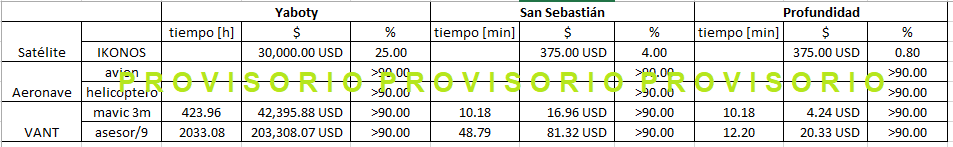
\includegraphics[width=\textwidth]{Imagenes/Tabla comparativa borrador.png}
     \hfill
     %\caption{Supe}
        \label{Tabla}
\end{figure}
Obtener los datos y características técnicas de los sensores no es tarea sencilla. La información que suele figurar en los sitios web de los fabricantes o en los manuales, no suele ser la que se necesita para calcular. Por ejemplo la distancia focal no suele ser un dato que aparezca en la lista de especificaciones. Puede obtenerse de los metadatos asociados a una imagen que ha sido capturada con ese sensor.
Del mismo modo tampoco resulta sencillo obtener información sobre las tarifas de vuelos de relevamiento aéreo, ya sea tripulado o no. La información disponible es vaga y escueta, por ejemplo la hora de vuelo tripulado es de 240 dólares estadounidenses si se toma como base el dólar oficial (cotizado en 55 mil pesos argentinos, mayo 2023), y la de VANT es de 195 dólares estadounidenses (cotizado en 45 mil pesos argentinos, mayo 2023).
\subsubsection{Hardware}
Los que se pueden seleccionar con mayor grado de libertad son los que están relacionados con el hardware asociado a la tarea, como es el sensor de la cámara, o las características de funcionamiento de la aeronave no tripulada. Una cámara con mayor resolución demandará mayor espacio de almacenamiento. Asimismo si se trata de sensores ópticos en el rango del espectro visible, la posibilidad de operar se limitará a las horas diurnas. No así si se trata de sensores que trabajan en otro rango de longitudes de onda, como los infrarrojos, o sensores activos, como LiDAR.
\subsubsection{Marco regulatorio}

\subsubsection{Almacenamiento necesario}
Dependiendo de la resolución espacial y espectral de las imágenes, los requerimientos de almacenamiento aumentarán en proporción a las mismas. Siguiendo con el ejemplo antes expuesto, las casi seis millones y medio de fotografías en RGB, con 5 Megapíxeles por cada una, con una profundidad de color de 8 bit por canal necesitarían un espacio de almacenamiento de alrededor de 7,5 Terabytes.
\subsubsection{Cálculo presupuestario}
Partiendo de las características del terreno a relevar (su extensión) y de la plataforma usada para la captura (dron con cámara/sensor) es posible acotar un marco presupuestario para llevar a cabo la tarea. Con los datos recabados puede afirmarse que para un relevamiento aéreo de un área pequeña de veinte hectáreas, es conveniente un VANT, ya que el costo total no excedería los 10 dólares, mientras que en un avión tripulado el costo total sería por lo menos diez veces, y una imagen satelital tendría un costo de 375 dólares. En el caso de un área un poco más grande, de cien hectáreas, el costo total con VANT sigue siendo más bajo que con las otras plataformas, con menos de 50 dólares. Finalmente para el caso de un área mucho más grande, de varios miles de hectáreas como la reserva Yaboty, se torna más conveniente el avión tripulado con alrededor de 20 mil dólares estadounidenses, un poco más que la mitad de lo que cuesta la imagen satelital, y muy por debajo del costo del VANT, que supera holgadamente el millón de dólares.
%%%%%%%%%%%%%%%%%%%%%%%%%%%%%%%%%%%%%%%%% TABLA %%%%%%%%%%%%%%%%%%%%%%%%%%%%%%%%%%%%%%%%%%%%%%%%%%%%%%%%%
% Please add the following required packages to your document preamble:
% \usepackage{multirow}
% \usepackage[table,xcdraw]{xcolor}
% If you use beamer only pass "xcolor=table" option, i.e. \documentclass[xcolor=table]{beamer}
% \usepackage[normalem]{ulem}
% \useunder{\uline}{\ul}{}
% Please add the following required packages to your document preamble:
% \usepackage{multirow}
% \usepackage[table,xcdraw]{xcolor}
% If you use beamer only pass "xcolor=table" option, i.e. \documentclass[xcolor=table]{beamer}
% \usepackage[normalem]{ulem}
% \useunder{\uline}{\ul}{}
% Please add the following required packages to your document preamble:
% \usepackage{multirow}
% \usepackage[table,xcdraw]{xcolor}
% If you use beamer only pass "xcolor=table" option, i.e. \documentclass[xcolor=table]{beamer}
% \usepackage[normalem]{ulem}
% \useunder{\uline}{\ul}{}
% Please add the following required packages to your document preamble:
% \usepackage{multirow}
% \usepackage[table,xcdraw]{xcolor}
% If you use beamer only pass "xcolor=table" option, i.e. \documentclass[xcolor=table]{beamer}
% \usepackage[normalem]{ulem}
% \useunder{\uline}{\ul}{}
% Please add the following required packages to your document preamble:
% \usepackage{booktabs}
% \usepackage{graphicx}
% Please add the following required packages to your document preamble:
% \usepackage{booktabs}
% \usepackage{graphicx}
% Please add the following required packages to your document preamble:
% \usepackage{booktabs}
% \usepackage{multirow}
% \usepackage{graphicx}
% Please add the following required packages to your document preamble:
% \usepackage{multirow}
% \usepackage{graphicx}
% Please add the following required packages to your document preamble:
% \usepackage{multirow}
% \usepackage{graphicx}
% \usepackage[table,xcdraw]{xcolor}
% If you use beamer only pass "xcolor=table" option, i.e. \documentclass[xcolor=table]{beamer}
\begin{landscape}
\begin{table}[]

    \caption{Comparación de los tiempos y costos para cada plataforma}
    \label{tab:tabla}
   
    \begin{tabular}{cc|ccc|ccc|ccc|c|}
    \cline{3-12}
    \multicolumn{2}{c|}{} &
      \multicolumn{3}{c|}{\cellcolor[HTML]{68CBD0}\textbf{Yaboty}} &
      \multicolumn{3}{c|}{\cellcolor[HTML]{68CBD0}\textbf{San   Sebastián}} &
      \multicolumn{3}{c|}{\cellcolor[HTML]{68CBD0}\textbf{Profundidad}} &
       \\ \cline{3-11}
    \multicolumn{2}{c|}{\multirow{-2}{*}{}} &
      \multicolumn{1}{c|}{\cellcolor[HTML]{68CBD0}\textit{Tiempo {[}h{]}}} &
      \multicolumn{1}{c|}{\cellcolor[HTML]{68CBD0}\textit{\$}} &
      \cellcolor[HTML]{68CBD0}\textit{\%} &
      \multicolumn{1}{c|}{\cellcolor[HTML]{68CBD0}\textit{Tiempo {[}min{]}}} &
      \multicolumn{1}{c|}{\cellcolor[HTML]{68CBD0}\textit{\$}} &
      \cellcolor[HTML]{68CBD0}\textit{\%} &
      \multicolumn{1}{c|}{\cellcolor[HTML]{68CBD0}\textit{Tiempo {[}min{]}}} &
      \multicolumn{1}{c|}{\cellcolor[HTML]{68CBD0}\textit{\$}} &
      \cellcolor[HTML]{68CBD0}\textit{\%} &
      \multirow{-2}{*}{\textbf{Resolución espacial {[}cm/pixel{]}}} \\ \hline
    \multicolumn{1}{|c|}{\cellcolor[HTML]{9698ED}} &
      \cellcolor[HTML]{9698ED}Pleiades &
      \multicolumn{1}{c|}{} &
      \multicolumn{1}{c|}{37,500.00 USD} &
       &
      \multicolumn{1}{c|}{} &
      \multicolumn{1}{c|}{375.00 USD} &
       &
      \multicolumn{1}{c|}{} &
      \multicolumn{1}{c|}{375.00 USD} &
       &
       \\ \cline{2-12} 
    \multicolumn{1}{|c|}{\cellcolor[HTML]{9698ED}} &
      \cellcolor[HTML]{9698ED}Satellogic &
      \multicolumn{1}{c|}{} &
      \multicolumn{1}{c|}{37,500.00 USD} &
       &
      \multicolumn{1}{c|}{} &
      \multicolumn{1}{c|}{375.00 USD} &
       &
      \multicolumn{1}{c|}{} &
      \multicolumn{1}{c|}{375.00 USD} &
       &
       \\ \cline{2-12} 
    \multicolumn{1}{|c|}{\multirow{-3}{*}{\cellcolor[HTML]{9698ED}\textbf{Satélite}}} &
      \cellcolor[HTML]{9698ED}IKONOS &
      \multicolumn{1}{c|}{} &
      \multicolumn{1}{c|}{37,500.00 USD} &
      ? &
      \multicolumn{1}{c|}{} &
      \multicolumn{1}{c|}{375.00 USD} &
      4.00 &
      \multicolumn{1}{c|}{} &
      \multicolumn{1}{c|}{375.00 USD} &
      0.80 &
      96.35 \\ \hline
    \multicolumn{1}{|c|}{\cellcolor[HTML]{9698ED}} &
      \cellcolor[HTML]{9698ED}Ala fija &
      \multicolumn{1}{c|}{69.13} &
      \multicolumn{1}{c|}{6,912.77 USD} &
      \textgreater{}90.00 &
      \multicolumn{1}{c|}{2.24} &
      \multicolumn{1}{c|}{3.74 USD} &
      \textgreater{}90.00 &
      \multicolumn{1}{c|}{0.42} &
      \multicolumn{1}{c|}{0.70 USD} &
      \textgreater{}90.00 &
      10.21 \\ \cline{2-12} 
    \multicolumn{1}{|c|}{\multirow{-2}{*}{\cellcolor[HTML]{9698ED}\textbf{Aeronave}}} &
      \cellcolor[HTML]{9698ED}Ala rotativa &
      \multicolumn{1}{c|}{} &
      \multicolumn{1}{c|}{} &
      \textgreater{}90.00 &
      \multicolumn{1}{c|}{} &
      \multicolumn{1}{c|}{} &
      \textgreater{}90.00 &
      \multicolumn{1}{c|}{} &
      \multicolumn{1}{c|}{} &
      \textgreater{}90.00 &
       \\ \hline
    \multicolumn{1}{|c|}{\cellcolor[HTML]{9698ED}} &
      \cellcolor[HTML]{9698ED}mavic 3m &
      \multicolumn{1}{c|}{8645.64} &
      \multicolumn{1}{c|}{ 1,685,899.92  USD} &
      \textgreater{}90.00 &
      \multicolumn{1}{c|}{5.12} &
      \multicolumn{1}{c|}{8.53 USD} &
      \textgreater{}90.00 &
      \multicolumn{1}{c|}{1.22} &
      \multicolumn{1}{c|}{2.04 USD} &
      \textgreater{}90.00 &
      10.23 \\ \cline{2-12} 
    \multicolumn{1}{|c|}{\cellcolor[HTML]{9698ED}} &
      \cellcolor[HTML]{9698ED}asesor/9 &
      \multicolumn{1}{c|}{21666.57} &
      \multicolumn{1}{c|}{ 4,224,981.67 USD } &
      \textgreater{}90.00 &
      \multicolumn{1}{c|}{10.38} &
      \multicolumn{1}{c|}{17.30 USD} &
      \textgreater{}90.00 &
      \multicolumn{1}{c|}{2.19} &
      \multicolumn{1}{c|}{3.66 USD} &
      \textgreater{}90.00 &
      5.34 \\ \cline{2-12} 
    \multicolumn{1}{|c|}{\multirow{-3}{*}{\cellcolor[HTML]{9698ED}\textbf{VANT}}} &
      \cellcolor[HTML]{9698ED}mini 2 &
      \multicolumn{1}{c|}{18854.06} &
      \multicolumn{1}{c|}{ 3,676,541.38 USD } &
      \textgreater{}90.01 &
      \multicolumn{1}{c|}{9.34} &
      \multicolumn{1}{c|}{15.57 USD} &
      \textgreater{}90.01 &
      \multicolumn{1}{c|}{2.25} &
      \multicolumn{1}{c|}{3.75 USD} &
      \textgreater{}90.01 &
      3.47 \\ \hline
    \end{tabular}%

\end{table}
\end{landscape}
%%%%%%%%%%%%%%%%%%%%%%%%%%%%%%%%%%%%%%%%%%%%%%%%%%%%%%%%%%%%%%%%%%%%%%%%%%%%%%%%%%%%%%%%%%%%%%%%%%%%%%%%%

\section{ Propuesta de Herramientas de Bajo Costo (Económico y Computacional) para el relevamiento del bosque atlántico}
\subsection{A2-Relación de iluminación natural con histogramas de color}
Con el objeto de evaluar la correspondiente afectación en el histograma de las imágenes capturadas respecto a las condiciones de iluminación natural, se hicieron varias capturas en distintos horarios durante varios días desde una posición fija a un determinado objeto (un árbol de palta) y se midió la iluminancia usando un luxómetro.
\subsection{B-Replicación del paper de Wagner}
A partir de un trabajo publicado por \cite{hubert_wagner_individual_2018}, se intentó replicar una parte del mismo que implementaba una serie de procedimientos morfológicos a una imagen aérea o satelital en escala de grises de una porción de selva, para delinear copas individuales previo a realizar una clasificación de especies.
\subsection{C1-Lógica difusa y procesamiento homomórfico (sombras)}
Según el modelo Stockham \cite{stockham_image_1972} una imagen puede descomponerse en dos partes, una la denominada iluminación y la otra componente es la reflexión. Llevadas al plano de frecuencias, se confirma el hecho de que la componente de iluminación tiene una variación más lenta, es decir, se corresponde con las frecuencias bajas. De modo similar, la componente de reflexión se corresponde con frecuencias altas \cite{oppenheim_nonlinear_1968}. Entendiendo esto, es factible implementar un filtrado en la imagen para realzar las sombras, separando la componente de iluminación de la de reflexión. Esta técnica fue utilizada en la remoción de sombras en imágenes de piezas de manufactura \cite{yang_research_2012} y en la detección automática de sombras en objetos oscuros \cite{etemadnia_automatic_2003}. En el presente trabajo, la aplicación a la detección de especies arbóreas es novedosa. 
Tomando como base el modelo de iluminación de Stockham para descomponer partes iluminadas de sombreadas, adoptando el concepto de frecuencia espacial, se implementó un procedimiento que incluía una etapa de filtrado homomórfico seguida de una etapa de aplicación de lógica difusa para discriminar sombras en imágenes aéreas de porciones de selva.
La imagen se modela como el producto de una componente de iluminación y otra de reflexión, que depende de las características del objeto iluminado. 
La ecuación que representa al filtro es
%%%%%%%%%%%%%%%%%%%%%%%%%%%%%%%%%%%%%% ECUACIÓN %%%%%%%%%%%%%%%%%%%%%%%%%%%%%%%%%%%%%%%%%%%%%%%%%%%%%%%%%
\\
\begin{equation}
	H(u,v)=1-((\gamma_H-\gamma_L)(1-e^{\frac{-cD^L(u,v)}{D^L_0}}+\gamma_L),\label{filtro homomorfico}
\end{equation}
\\
%%%%%%%%%%%%%%%%%%%%%%%%%%%%%%%%%%%%%%%%%%%%%%%%%%%%%%%%%%%%%%%%%%%%%%%%%%%%%%%%%%%%%%%%%%%%%%%%%%%%%%%%%  


donde $D_0$ es la frecuencia de corte, $c$ controla la forma y pendiente del filtro en la región de trancisión entre $\gamma_L$ y $\gamma_H$. $D(u,v)$ es la distancia al origen del plano de frecuencias.

Las imágenes a ser analizadas fueron obtenidas desde el sitio web Bing (poner en referencia de la dirección web del maps). Se seleccionaron imágenes de diferentes sitios de la Provincia de Misiones, correspondientes a selvas en parques y reservas, en los que se supone mayor presencia de especies de árboles de interés para el presente trabajo. 
En un primer paso se realizó la conversión de la imagen de color rojo, verde y azul (RGB) a la representación matiz, saturación e intensidad (HSI), trabajando sobre la componente de intensidad. En un paso siguiente se aplicó el logaritmo a la componente de intensidad de la imagen y seguidamente se obtuvo la transformada de Fourier de la misma, para poder procesar con el filtro de sombras. Se multiplicó la matriz de la imagen por la matriz que representa al filtro y, luego, al resultado se aplicó la transformada inversa de Fourier, la función inversa de logaritmo y la remoción de fase, tomando el módulo del número complejo, todo en orden sucesivo. Posteriormente se binarizó la imagen filtrada mediante un criterio de umbral de 0,75 en una escala en la que el valor 1 es blanco y 0 es negro. La imagen de salida del filtro de sombras presenta a las sombras resaltadas con píxeles de intensidad blancos. 
Luego se efectuó la selección de las sombras binarizadas, con lo que se descartaron las sombras que no revisten interés para el posterior conteo, estableciendo una ventana de enmascaramiento, que a los efectos prácticos es cuadrada y el criterio de clasificación es de 45\% de píxeles blancos. Una vez completas la binarización y la selección de sombras de interés, se realizó el conteo de las mismas. El diagrama de flujo de la fig. 3 describe las etapas del proceso completo. A los efectos de demostrar el grado de certeza del algoritmo, se comparó con la detección manual, variando el tamaño de la ventana de enmascaramiento. Se comprobó que eligiendo un tamaño de ventana de enmascaramiento igual a 20 por 20 píxeles se obtenía un acercamiento al criterio de selección manual.
En el proceso de binarización, se definió como umbral que correspondía a un valor de intensidad por encima del cual se trataba de sombras. En este caso el valor de intensidad fue de 0,75 en valores de intensidad de píxeles normalizados.
Para la selección de sombras binarizadas se recorrió la matriz de la imagen con una ventana de inspección que abarcaba 25 píxeles por lado, de modo que se evalúa un conjunto de 625 píxeles. Se estableció un umbral de 0,45 para clasificar las sombras, de modo que los recintos de píxeles blancos que superaban ese umbral eran catalogados como sombras de árboles grandes.
A los efectos de mostrar el funcionamiento del método de búsqueda y conteo de sombras, se exponen las fig. 4, 5 y 6 en las que se visualizan la imagen satelital en escala de grises de una porción de la reserva privada Sombra de Toro, ubicada en el norte de la provincia de Misiones, la imagen binarizada luego del filtrado homomórfico y las sombras seleccionadas, respectivamente.

\subsubsection{RESULTADOS}
Los resultados de las pruebas se exponen en la Tabla I. Allí se visualiza para distintas imágenes la cantidad de sombras detectadas, y se comparan los resultados de conteo automático con distintos tamaños de ventana, con el método de búsqueda de forma manual. Nótese el cambio de signo para el error medio entre los tamaños de ventana de 25 y de 20 píxeles, indicando que la selección de un tamaño de ventana menor resultará en una mayor 
cantidad de sombras detectadas que la que se obtiene por conteo manual. En cambio un tamaño de ventana mayor podría obviar varias sombras que serían tenidas en cuenta para el conteo manual. De acuerdo con la resolución de las imágenes de prueba, el tamaño de ventana cuadrada de 20 píxeles por lado se correspondería con un área de 100 metros cuadrados.

\subsubsection{CONCLUSIONES}
Los resultados de las pruebas indican que para el conteo de sombras deben considerarse varios factores. En principio la baja calidad de las imágenes utilizadas para las pruebas era evidente, y necesariamente debería hacerse un preprocesamiento de las imágenes, como ser ajustes y ecualizaciones de las componentes de color, para mejorar el contraste. Otra limitación para el uso de ésta técnica para el conteo de ejemplares de A. polyneuron es que debe reforzarse la contundencia de la afirmación de que esas sombras seleccionadas son efectivamente de dicha especie. Al no disponer de los datos asociados a las imágenes como ser fecha y hora exacta de la captura, se hacía difícil discernir si las sombras correspondían a árboles altos, o las sombras eran más intensas por el horario en el que fueron capturadas las imágenes (por ejemplo, en el crepúsculo) Hay que mencionar también las diferencias que hubo entre la detección de sombras por parte del algoritmo y la detección manual. Para el caso de la búsqueda automática con tamaño de ventana de 20 píxeles hubo casos de detección de falsos positivos, es decir, detectaba sombras donde el ojo humano no lo hacía, y también omitía seleccionar sombras que a simple vista serían consideradas como sombras de interés. Cabe añadir que la limitación de facto para el algoritmo es que realiza la selección de sombras con base en la observación de la componente intensidad del modelo HSI. Al ojo humano le resulta más fácil distinguir sombras en imágenes a color.

\subsection{C2-Índice invariante de color (sombras)}
Un método que dio resultados interesantes en la detección de sombras es el que implementaba el cálculo del índice invariante de color (IIC). Probando con distintos valores de umbral, se observó que el que producía resultados más satisfactorios era el que correspondía al 85º percentil de la distribución de los valores de IIC.
El punto de partida del método es la adquisición de imágenes aéreas. No hay requerimientos especiales, excepto que se den las condiciones para proyección de sombras. Se tomaron imágenes de un área representativa de la selva nativa en la provincia de Misiones, las cuales fueron capturadas desde un VANT que sobrevoló las áreas de interés. A los efectos de obtener imágenes con presencia de sombras, se estableció un adecuado rango temporal de captura de imagenes, en este caso de 3 a 4 pm. Las imágenes fueron adquiridas en el invierno meridional, en el mes de agosto, cuando la proyección de sombras es mayor debido a la posición relativa del sol. Se utilizó un dron Mini 2, del fabricante DJI, equipado con una cámara de 12 megapíxeles. La altura de vuelo sobre el terreno fue de 50 metros. la resolución espacial de las imágenes son de 3 cm/píxel.
\subsubsection{Introducción}
La conservación de áreas naturales forestales tiene cada vez mayor relevancia a nivel mundial debido a que los bosques nativos tienen un rol probado en la mitigación del cambio climático. En ese sentido se han propuestos numerosas acciones usando diversas herramientas para ayudar a conservar los bosques. Entre dichas herramientas el relevamiento y monitoreo de bosques mediante imágenes aéreas es un campo promisorio. En particular el monitoreo de la Selva Atlántica es un tópico que ha recibido mucha atención en las últimas décadas, desgraciadamente porque se ha convertido en uno de los ecosistemas más amenazados en el mundo. Siendo originalmente de una extensión de 1.290.692,46 km$^2$ durante los últimos siglos, que abarcaba parte de Brasil, Argentina y Paraguay, hoy la Selva Atlántica está reducida a casi 162.000 km$^2$, lo que representa sólo un 12,4 \% de la extensión original \cite{de_lima_erosion_2020}, y se ubica principalmente en la Provincia de Misiones en Argentina. A pesar de de este escenario adverso, la diversidad de especies que habitan en la Selva Atlántica es aún una de las más grandes del mundo \cite{lima_how_2015}. Sin embargo algunas especies de fauna y flora están en un estado de conservación crítico, como por ejemplo algunas especies de árboles cuya copa sobresale del dosel, situándose en lo que se conoce como capa emergente, a treinta metros o más respecto del suelo \cite{noauthor_rainforest_2015}, por lo que sería recomendable conocer la cantidad y geolocalización de este tipo de árboles. También sería de interés determinar la distribución y localización de algunas especies como bambú y lianas, que podrían ser indicadores de niveles de preservación \cite{bedrij_selective_2022}. En este contexto el monitoreo forestal representa un rol crítico en la evaluación de la eficacia de estrategias de restauración, identificando acciones correctivas, comparando resultados entre proyectos y aprendiendo de proyectos pasados para determinar futuros lineamientos en restauración \cite{viani_protocol_2017}
El nivel de preservación de la Selva Atlántica ha sido evaluado con varios métodos. El más difundido es la exploración in situ, restringido a áreas pequeñas, con posibilidad de ser extrapolados los resultados a áreas más grandes con el correspondiente error de estimación. En esta forma tradicional, el monitoreo forestal es una tarea ardua y demandante de tiempo, por lo que al transcurrir el tiempo entre revisitas, las condiciones ambientales podrían haber cambiado de modo considerable. Además el desplazamiento dentro de la selva resulta difícil y puede generar disturbios en la flora y en la fauna locales. Todo esto puede evitarse con el monitoreo forestal por medio de análisis de imágenes aéreas o satelitales. Éstas últimas representan una fuente interesante de datos, principalmente debido al inmenso área que puede cubrir una simple escena (cientos de kilómetros cuadrados) con múltiples bandas espectrales, especialmente más allá del espectro visible. Sin embargo tienen usualmente una relativamente baja resolución espacial y baja disponibilidad. En el mejor de los casos la resolución espacial de estas imágenes está en el orden de 30 cm por pixel \cite{poli_radiometric_2014}, siendo su adquisición onerosa, que puede ser de varios miles de dólares por cada escena \cite{noauthor_geocento_2022}. La obtención de estas imágenes está condicionada a la disponibilidad en el tiempo, ya que en algunos casos la frecuencia de revisita de determinados sitios puede ser de varios días \cite{li_global_2017}.
A pesar de estas desventajas, varios trabajos han relevado especies arbóreas y recolectado datos forestales usando imágenes satelitales con alta resolución espacial y espectral \cite{gomes_detection_nodate,cross_classification_2019,abd_latif_determination_2012,ferreira_tree_2019,radoux_quantitative_2007}. Por otro lado, otros trabajos han monitoreado bosques usando otras herramientas como los vehículos aéreos no tripulados (VANT) \cite{albuquerque_remotely_2020,albuquerque_forest_2021,qin_individual_2022,machida_modeling_2022}, en la detección de flores \cite{campbell_simple_2018} o incorporando sensores LiDAR \cite{terryn_quantifying_2022,brede_non-destructive_2022}. La combinación de imágenes aéreas o satelitales de alta resolución espacial con herramientas computacionales facilita la implementación del mapeo del estado de salud forestal \cite{prost_discrimination_2008} o el conteo automático de árboles \cite{putra_automatic_2023}. Las imágenes aéreas obtenidas con VANT poseen algunas ventajas sobre las satelitales, entre las que se encuentra su relativo bajo costo, su muy alta resolución espacial y su baja altitud de sobrevuelo, lo cual permite evitar interferencias de nubes \cite{alexander_locating_2018,ahmad_aerial_2010,zhang_seeing_2016,ahmad_digital_2013,colomina_unmanned_2014,eisenbeiss_mini_nodate}. No obstante, la combinación de la posibilidad de captura de imágenes de grandes extensiones de selva con una adecuada resolución espacial para luego procesar esas imágenes con métodos y tecnologías que ofrecen resultados aceptables sin excesivas demandas computacionales y requerimientos tecnológicos no es tan sencilla de implementar. La clave para alcanzar esa meta es trabajar con un atributo de la imagen que puede ser extraído con algoritmos eficientes. En este estudio asumimos que puede explorarse la información contenida en regiones sombreadas de imágenes aéreas de regiones forestales mediante algoritmos computacionales de bajo costo.
Las sombras se producen por oclusión por parte de un objeto de forma total o parcial de la luz directa emanada de la fuente \cite{hu_revisiting_2021}. En la bibliografía se considera que las sombras en imágenes de sensado remoto pueden ser originados por tres causas: material natural o urbano (árboles o edificios), características topográficas (colinas o montañas) y nubes \cite{shahtahmassebi_review_2013}. La presencia de sombras en imágenes de sensado remoto es objeto de muchas consideraciones. En algunos casos las sombras pueden ser una fuente de información útil, proveyendo por ejemplo una perspectiva en tres dimensiones de una escena capturada, mientras que en otros casos la presencia de sombras dificulta la recolección de datos detallados. Hay por lo tanto numerosos trabajos sobre el procesamiento de imágenes con sombras \cite{shahtahmassebi_review_2013,mostafa_review_2017,freitas_automatic_2017,chang_c_evaluation_2016}. Algunos trabajos están basados en el modelo de Stockham \cite{stockham_image_1972}, implementando el filtrado homomórfico para la remoción de sombras \cite{yang_shadow_2007} o para la detección de sombras en imágenes aéreas de selvas \cite{bernhardt_deteccion_2017}. Para la detección de sombras puede utilizarse como base la invariancia de color \cite{gevers_content-based_1999,geusebroek_color_2001}. En el presente trabajo nos enfocamos en el procedimiento de detección de sombras partiendo de tres hipótesis, la primera de las cuales es que las sombras que son causadas por depresiones en el dosel selvático y por la presencia de especímenes de capa emergente pueden ser detectadas de manera automática en las imágenes aéreas. La segunda hipótesis es que se puede utilizar índices invariantes de color para obtener una clasificación de píxeles de la imagen según corresponda a una región sombreada o no. Y la tercera hipótesis es que ciertas características presentes en el histograma de la imagen permiten automatizar la determinación de el umbral para binarizar la imagen en sendas regiones, sombreadas y no sombreadas.
En resumen, la propuesta del presente estudio es un método de detección automática de sombras en imágenes aéreas de selvas, basado en el cálculo del índice invariante de color \cite{sirmacek_damaged_2009} que se obtiene al combinar dos de los tres canales RGB de la imagen. Además la metodología propuesta demuestra la utilidad del percentil en la frecuencia de distribución del índice invariante de color para la obtención del umbral de binarización, lo cual permite la automatización de la segmentación de sombras en la imagen de un modo relativamente simple. El objetivo principal de este trabajo es obtener un método fiable para detección de sombras usando las fácilmente obtenidas y ampliamente difundidas imágenes RGB, con base en métodos computacionales poco demandante en cuanto a recursos.
Los detalles de la metodología propuesta se desarrollan en la sección \ref{Metodología}. La validación es descripta en \ref{Validacion}, y los resultados se muestran en \ref{Resultados}. Finalmente las conclusiones son discutidas en \ref{Conclusiones}
\subsubsection{Metodología propuesta}
En esta sección se describen los pasos del método de procesamiento necesarios para obtener la máscara automática de sombras de la imagen aérea. La figura \ref{diagrama_procesamiento} representa la secuencia de procesamiento.

\begin{figure}
    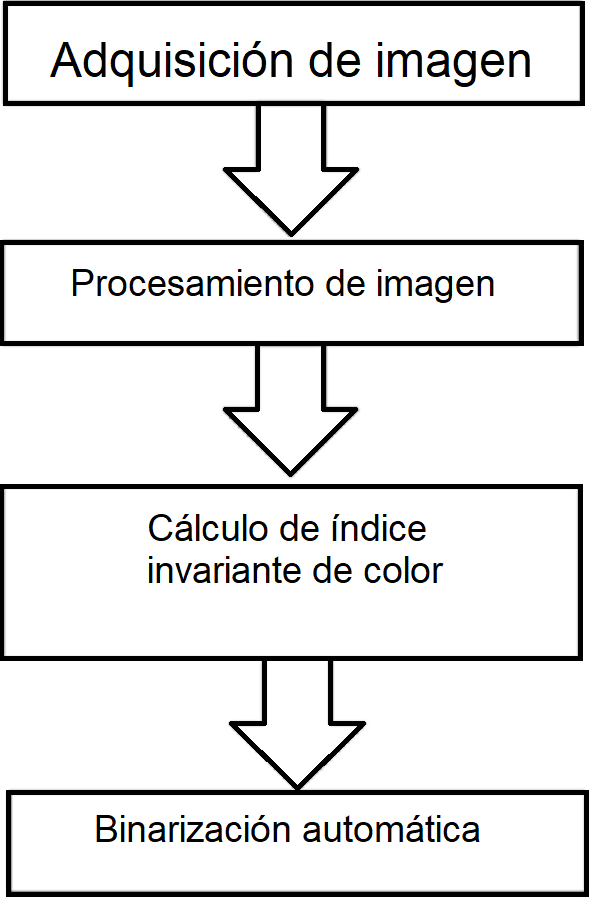
\includegraphics[width=\textwidth]{Imagenes/flowchart.png}
     \hfill
     \caption{Diagrama del procesamiento}
    \label{diagrama_procesamiento}
\end{figure}

\paragraph{Adquisición de la imagen}
El punto de partida de la metodología propuesta es la captura de imágenes aéreas. Entre los pocos requerimientos en esta etapa se destaca que las condiciones de luz solar deben ser las apropiadas para generar proyecciones de sombra. Aquí se consideran imagenes representativas de un área de selva nativa en la provincia de Misiones, Argentina, que han sido capturadas mediante VANT sobrevolando porciones de selva en parques y reservas naturales, en las cuales habría presencia de ejemplares de árboles de interés. Para garantizar una mejor captura de imágenes con sombra, se seleccionó un intervalo de tiempo que abarca desde las 3 p.m. hasta las 4 p.m., que es cuando la posición relativa del sol facilita la proyección de sombras sobre el dosel. Las imágenes fueron capturadas durante el invierno meridional, específicamente en el mes de agosto, cuando las sombras proyectadas son mayores para ese horario. Se usó un VANT modelo Mini 2 del fabricante DJI, equipado con una cámara con resolución de 12 Megapíxeles. La altura de vuelo sobre el terreno fue de 50 metros, y el modo en que estuvo configurada la cámara era automático. Las imágens capturadas están en formato JPG con una resolución de 4000 x 2250 píxeles, con una resolución espacial de 3 cm/pixel aproximadamente. Para ejecutar el algoritmo se usó una computadora laptop común con un procesador Intel Core i5. En cuanto a los scripts, están basados en códigos de Octave. Se analizó un total de 19 imágenes.

\paragraph{Preprocesamiento de imagen} \label{Metodología}
Para facilitar el procesamiento y posterior análisis, las imágenes de los diferentes sitios deben ser recortadas par anormalizar el tamaó y ser filtradas para estandarizar algunos atributos.
\paragraph{Cálculo de índice invariante de color}
Con base en imágenes filtradas RGB, el invariante de color $\Psi$ se calcula por medio de la ecuación \ref{invariante de color}
 %%%%%%%%%%%%%%%%%%%%%%%%%%%%%%%%%%%%%% ECUACIÓN %%%%%%%%%%%%%%%%%%%%%%%%%%%%%%%%%%%%%%%%%%%%%%%%%%%%%%%%%
\\
\begin{equation}
	\Psi=\frac{4}{\pi} arctan\left(\frac{B\textsubscript{1}-B\textsubscript{2}}{B\textsubscript{1}+B\textsubscript{2}}\right),\label{invariante de color}
\end{equation}
\\
%%%%%%%%%%%%%%%%%%%%%%%%%%%%%%%%%%%%%%%%%%%%%%%%%%%%%%%%%%%%%%%%%%%%%%%%%%%%%%%%%%%%%%%%%%%%%%%%%%%%%%%%%
 donde $B_1$ y $B_2$ son dos bandas diferentes de color, rojo, verde o azul. El índice invariante de color $\Psi$ toma un valor entre -1 y 1. Si se aplica la ecuación a las bandas correspondientes $B_1$ y $B_2$, el resultado es una matriz de idéntico tamaño al de la imagen, en la que cada píxel contiene el valor del índice invariante de color. Según sea la combinación entre bandas, hay hasta seis posibilidades, siendo una mitad complementaria de la otra mitad. Por esta razón sólo se tienen en cuenta tres de esas posibilidades. La matriz de índice invariante de color se usó para analizar las partes sombreadas y no sombreadas de la imagen. Así, para las tres combinaciones a implementar, se describen en las ecuaciones \ref{psibr}, \ref{psibg} y \ref{psigr}:
 \\
 \\
\begin{equation}
	\Psi_{BR}=\frac{4}{\pi} arctan\left(\frac{B\textsubscript{B}-B\textsubscript{R}}{B\textsubscript{B}+B\textsubscript{R}}\right),\label{psibr}
\end{equation}
\\
\\
\begin{equation}
	\Psi_{BG}=\frac{4}{\pi} arctan\left(\frac{B\textsubscript{B}-B\textsubscript{G}}{B\textsubscript{B}+B\textsubscript{G}}\right),\label{psibg}
\end{equation}
\\
\\
\begin{equation}
	\Psi_{GR}=\frac{4}{\pi} arctan\left(\frac{B\textsubscript{G}-B\textsubscript{R}}{B\textsubscript{G}+B\textsubscript{R}}\right),\label{psigr}
\end{equation}
\\
donde $B_{B}$, $B_{G}$, y $B_{R}$ son los canales azul, verde y rojo respectivamente.
\paragraph{Binarización automática}
 La binarización permite separar la imagen en dos regiones, con sombra y sin sombra, mediante la matriz de índice invariante de color y un valor de umbral, calculado como la frecuencia acumulada de la distribución de valores individuales de IIC. Esta máscara que se obtiene, denominada máscara automática, se compone de píxeles de valores 1 y 0, correspondiendo el valor de 1 al de las regiones sombreadas de la imagen. En la composición de la máscara binaria se asume un valor de 1 (visualizado en blanco) para las regiones sombreadas. Tomando la distribución de frecuencia acumulada del índice invariante de color, se determina el valor umbral que excede los percentiles 60º, 70º, 80º, 85º, 90º y 95º. De este modo, en el presente trabajo, se obtienen seis máscaras, cada una correspondiente al valor de umbral de cada percentil. Luego el valor de umbral es variable y es calculado para cada imagen para un percentil determinado. La calidad de cada máscara automática obtenida es evaluada al compararse con una máscara manual obtenida por un experto humano para la correspondiente imagen.

\paragraph{Comparación cuantitativa con un índice de calidad}
Para establecer un índice de calidad (QI) del desempeño de la selección automática, se proponen tres índices: el primero ($QI_1$) se obtiene del cociente entre la suma de todos los píxeles de la matriz binaria, obtenida como consecuencia de la intersección de la máscara manual y la máscara automática, y la suma de todos los elementos de la máscara manual (\ref{qi1}). El segundo índice ($QI_2$) se obtiene dividiendo la suma de elementos de la intersección por la suma de los elementos de la máscara automática (\ref{qi2}); y el tercer índice ($QI_3$) se obtiene dividiendo la suma de los elementos de la intersección por la suma de los elementos de la unión de la máscara manual y automática (\ref{qi3}.
\\
\\
 \begin{equation}
    QI_1=\frac{\Sigma _{i,j}(M_M\cap M_A )}{\Sigma _{i,j}(M_M ) }
    \label{qi1}
\end{equation}
\\
\\
 \begin{equation}
    QI_2=\frac{\Sigma _{i,j}(M_M\cap M_A )}{\Sigma _{i,j}(M_A ) }
    \label{qi2}
\end{equation}
\\
\\
\begin{equation}
    QI_3=\frac{\Sigma _{i,j}(M_M\cap M_A )}{\Sigma _{i,j}(M_M \cup M_A ) }
    \label{qi3}
\end{equation}
\\
\\
Donde $M_M$ es la máscara binaria manual y $M_A$ es la máscara binaria automática. Cada uno de los índices precedentes toma valores de 0 a 1, siendo 0 el caso en que no hay ninguna coincidencia entre máscaras, y 1 indica plena coincidencia. Para los tres índices, el numerador es la intersección entre ambas máscaras, manual y automática, ya que es un buen indicador de coincidencia entre ambas. El denominador en tanto da un valor de referencia que parametriza el índice. La intersección y la unión son operaciones lógicas que se aplican a cada píxel, de modo que es una condición necesaria que sendas máscaras binarias automática y manual que serán comparadas entre sí, sean del mismo tamaño y de áreas de captura coincidentes. En un nivel de píxel, la intersección es una operación lógica "and", por lo que, al ser cero uno de sendos píxeles comparados, el resultado de la operación dará cero. Por otro lado, la unión implica una operación a nivel de píxel de tipo "or", y siendo uno de sendos píxeles de valor uno, el resultado será uno. El objetivo de este índice es evaluar cuanto se asemeja la selección automática del algoritmo a la selección manual. Así, el mayor valor que corresponde a 1 implica una selección automática exacta, mientras que valores más bajos cercanos a cero corresponden a una pobre correlación entre sendas selecciones.


\paragraph{Etapa de filtrado}
Para quitar el ruido de la imagen, se implementa un filtro de mediana. Para evaluar cómo la etapa de filtrado afecta el desempeño de la selección automática, se realizaron para cada imagen tres pruebas con diferentes configuraciones de filtro, con vecindad de tres por tres, seis por seis, y  doce por doce pixeles. Para cada caso se propuso un conjunto de tres índices de calidad, descriptos en las ecuaciones \ref{qi5}, \ref{qi6} y \ref{qi7}
\\
\\
 \begin{equation}
    QI_5=\frac{\Sigma _{i,j}(M_{NF}\cap M_{WF})}{\Sigma _{i,j}(M_{NF}) }
    \label{qi5}
\end{equation}
\\
\\
 \begin{equation}
    QI_6=\frac{\Sigma_{i,j}(M_{NF}\cap M_{WF})}{\Sigma _{i,j}(M_{WF}) }
    \label{qi6}
\end{equation}
\\
\\
\begin{equation}
    QI_7=\frac{\Sigma _{i,j}(M_{NF}\cap M_{WF})}{\Sigma _{i,j}(M_{NF}\cup M_{WF}) }
    \label{qi7}
\end{equation}
\\
\\
en donde $M_{NF}$ es la máscara binaria automática obtenida sin filtrado, y $M_{WF}$ es la obtenida luego de la etapa de filtrado.

\subsubsection{Validación} \label{Validacion}
Superponiendo a una imagen las dos máscaras, una obtenida en forma manual y otra en forma automática, tres expertos realizaron un análisis, calificando el grado de ajuste entre ambas máscaras como "bueno", "regular" o "malo". Este procedimiento fue aplicado a cada una de las 19 imágenes analizadas, de modo que se obtuvieron 19 máscaras automáticas por medio del algoritmo para ser comparadas con las respectivas máscaras obtenidas en forma manual. Las superposiciones calificadas como "buenas" o "regulares" son usadas para seleccionar la mejor máscara automática. Un procedimiento similar se siguió para evaluar el filtrado de la imagen.

\subsubsection{Resultados} \label{Resultados}
Un total de diecinueve imágenes aéreas de selva fueron consideradas para realizar el análisis. Dos de ellas representativas de los diferentes escenarios que fueron cubiertos, se muestran en las figuras \ref{calle} y \ref{tupido}. La figura \ref{calle} muestra una imagen en la que unas pocas copas de árboles se distribuyen por el área capturada, mientras que en la \ref{tupido} el dosel cubre prácticamente toda el área. La delineación manual de las sombras fue realizada como se describe en el apartado de \ref{Metodología}
Dos ejemplos de máscaras manuales se muestran en figuras \ref{contorno1} y \ref{contorno2}, con trazo rojo bordeando las regiones sombreadas. La figura \ref{superposicion} muestra el solapamiento de la máscara manual (en rojo) con la automática (en azul). En la figura \ref{p60} el valor de umbral para la máscara binaria se toma del 60º percentil de la distribución de frecuencias, mientras que en la figura \ref{p85} el valor de umbral es tomado del 85º percentil.

\begin{figure}
    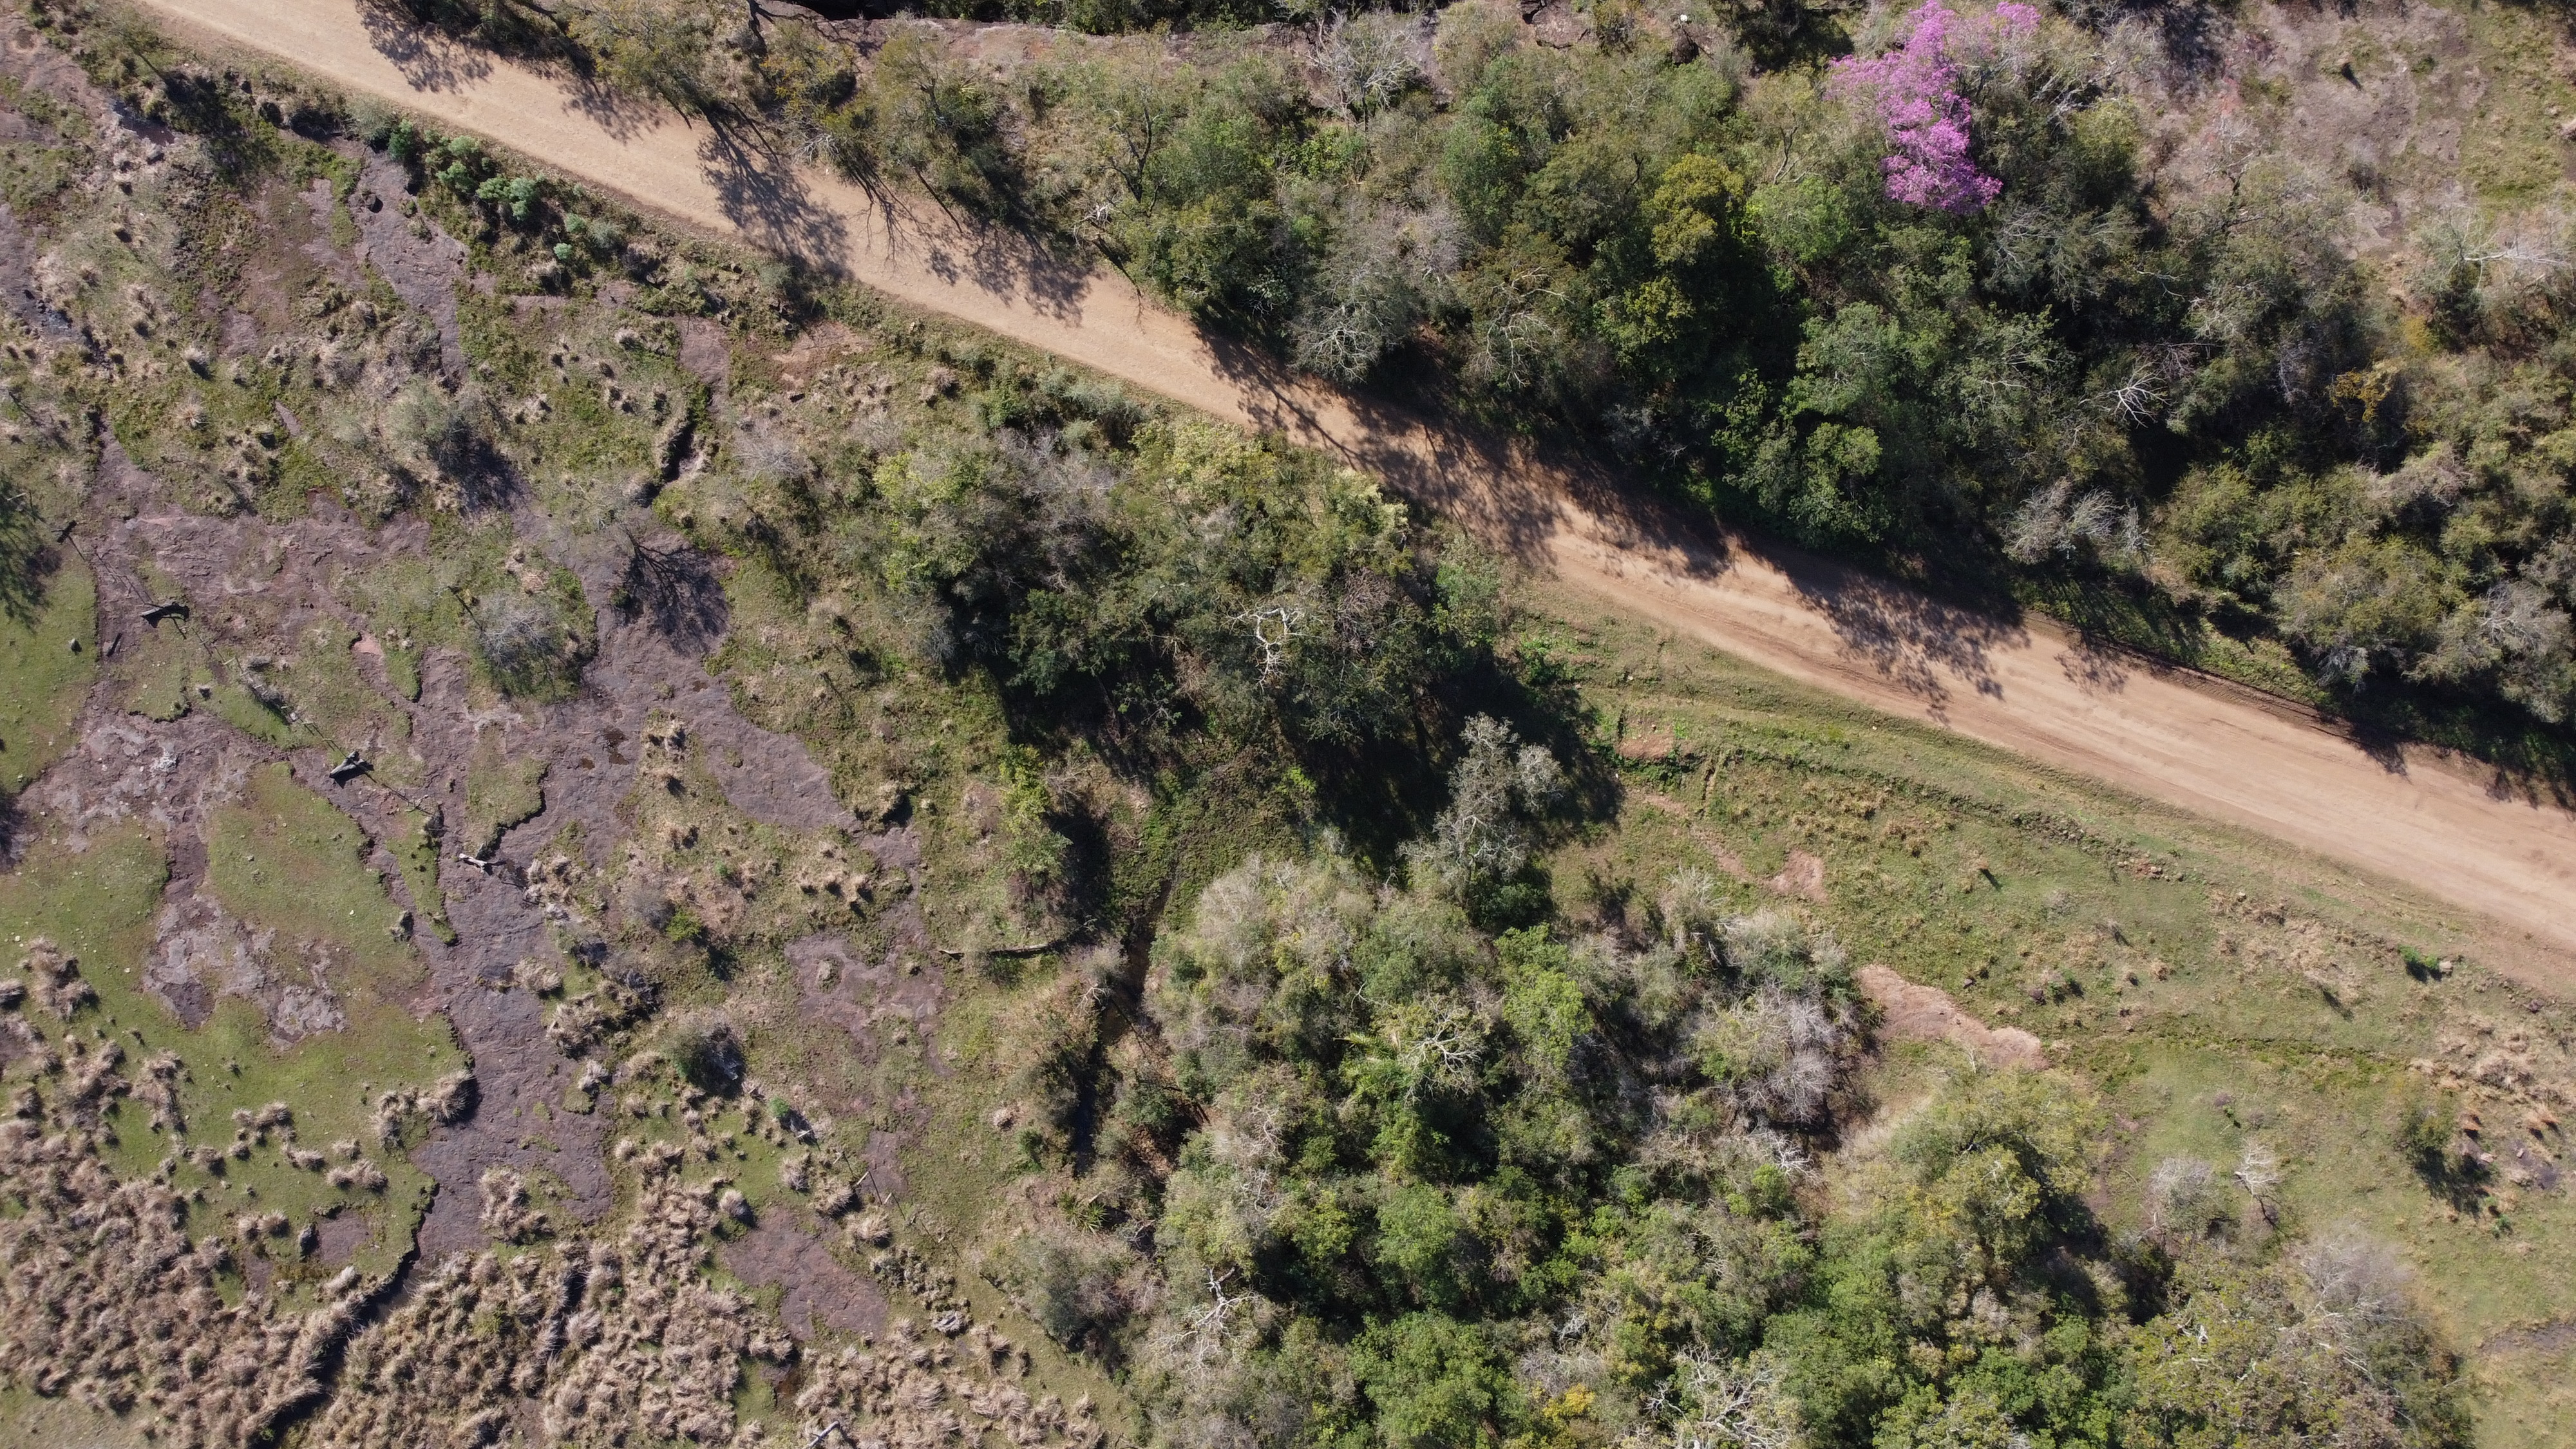
\includegraphics[width=\textwidth]{Imagenes/street.jpg}
     \hfill
     \caption{Escena capturada con pocos árboles}
    \label{calle}
\end{figure}

\begin{figure}
    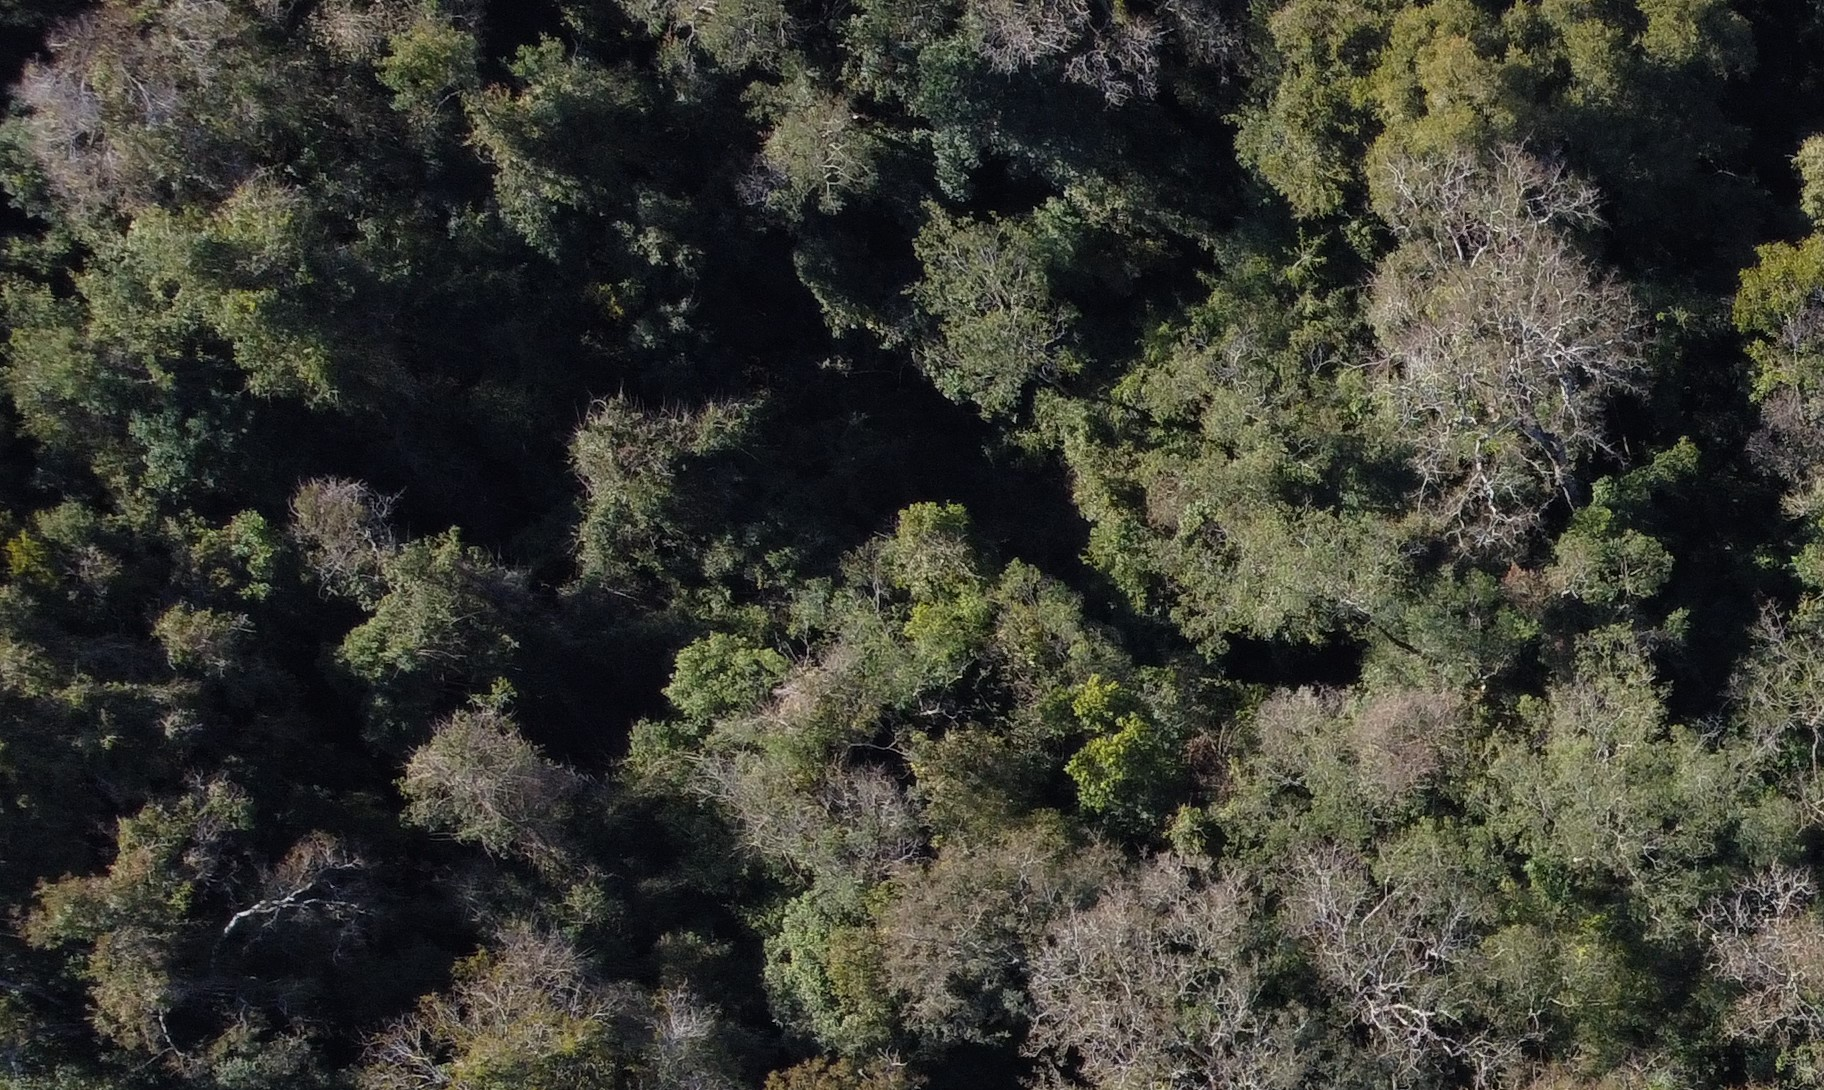
\includegraphics[width=\textwidth]{Imagenes/dense canopy.jpg}
     \hfill
     \caption{Escena capturada con dosel tupido}
    \label{tupido}
\end{figure}


\begin{figure}
    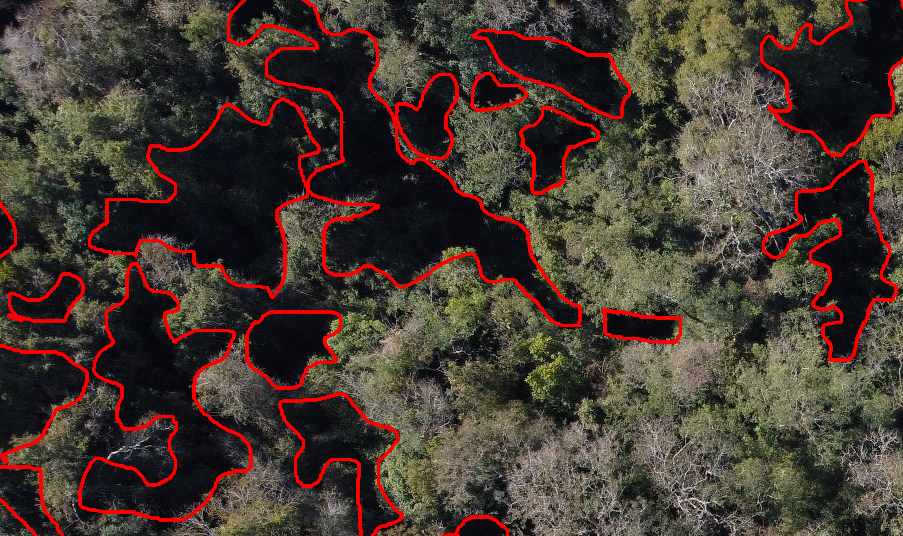
\includegraphics[width=\textwidth]{Imagenes/contours.png}
     \hfill
     \caption{Contornos de sombras en dosel tupido}
    \label{contorno1}
\end{figure}

\begin{figure}
    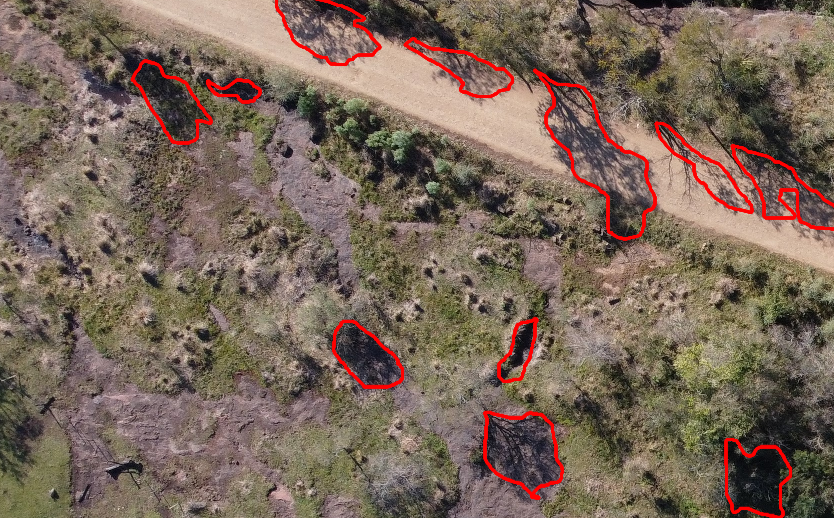
\includegraphics[width=\textwidth]{Imagenes/contours2.png}
     \hfill
     \caption{Contorno de sombras en imagen con pocos árboles}
    \label{contorno2}
\end{figure}

\begin{figure}
     \centering
     \begin{subfigure}[b]{0.5\textwidth}
         \centering
         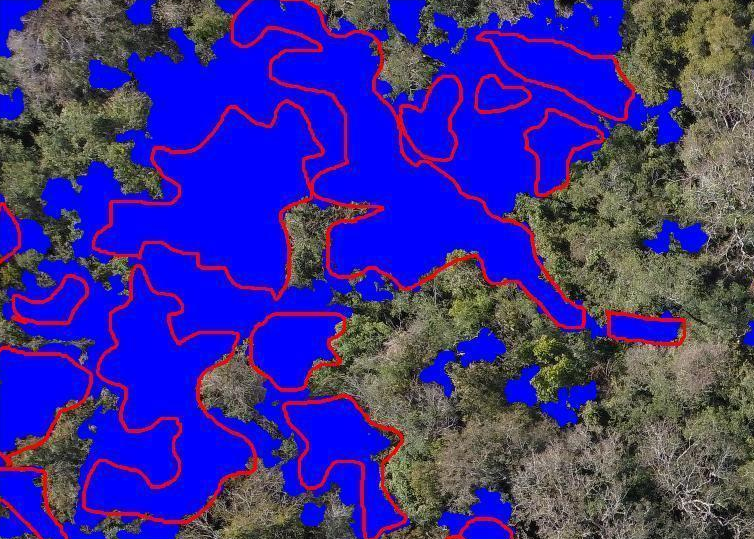
\includegraphics[width=\textwidth]{Imagenes/superposition of masks.png}
         \caption{Percentil 60º}
         \label{p60}
     \end{subfigure}
     \hfill
     
     \begin{subfigure}[b]{0.5\textwidth}
         \centering
         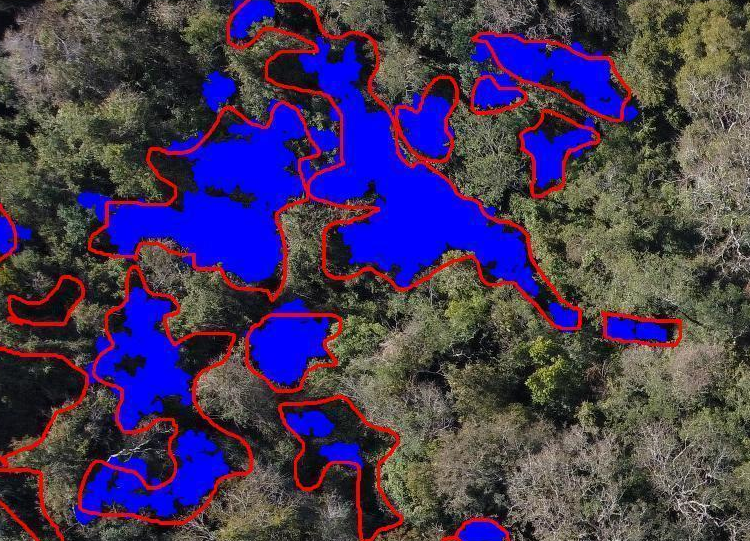
\includegraphics[width=\textwidth]{Imagenes/superposition of masks 2.png}
         \caption{Percentil 85º}
         \label{p85}
     \end{subfigure}
        \caption{Superposición de máscaras atuomática y manual}
        \label{superposicion}
\end{figure}

\begin{figure}
    \centering
  \begin{subfigure}[b]{0.3\textwidth}
    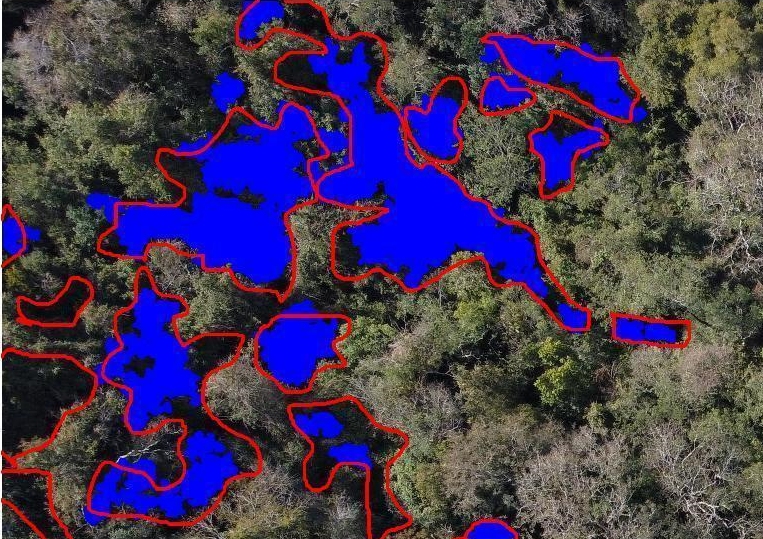
\includegraphics[width=\textwidth]{Imagenes/blue minus red 85.png}
     \hfill
     \caption{\textpsi\textsubscript{BR}}
    \label{azulrojo}
 \end{subfigure}

 \begin{subfigure}[b]{0.3\textwidth}
    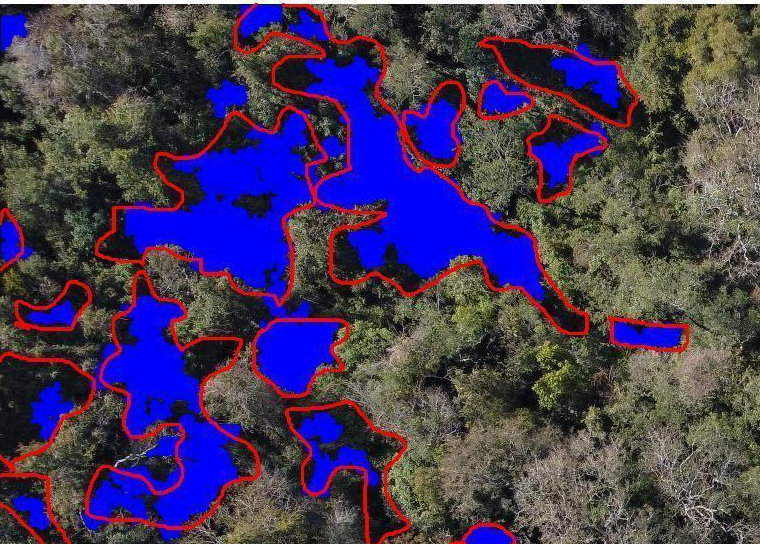
\includegraphics[width=\textwidth]{Imagenes/blue minus green 85.png}
     \hfill
     \caption{\textpsi\textsubscript{BG}}
    \label{azulverde}
 \end{subfigure}

 \begin{subfigure}[b]{0.3\textwidth}
    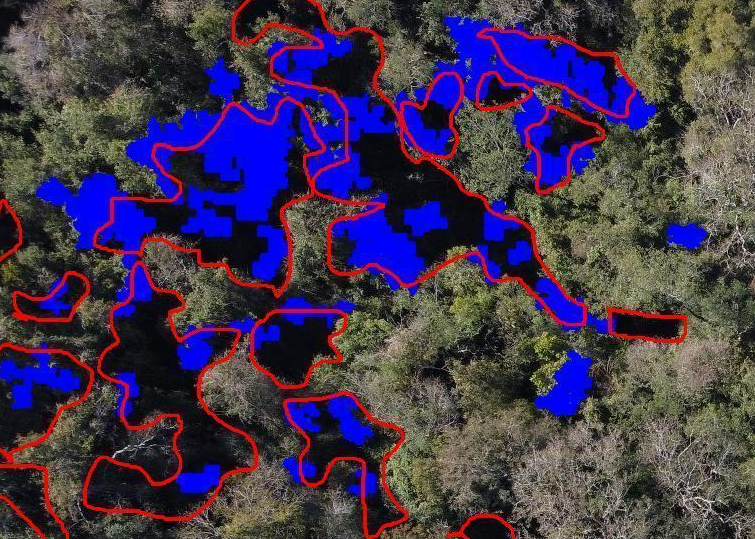
\includegraphics[width=\textwidth]{Imagenes/green minus red 85.png}
     \hfill
     \caption{\textpsi\textsubscript{GR}}
    \label{verderojo}
 \end{subfigure}
 \caption{Superposición de máscaras atuomática y manual}
        \label{p85BRBGGR}
\end{figure}

\paragraph{Influencia del valor de percentil y del índice invariante de color}

La figura \ref{azulrojo}, \ref{azulverde} y \ref{verderojo} muestra para la misma escena, diferentes máscaras automáticas obtenidas con diferentes configuraciones de la ecuación \ref{eq1}, usando tres diferentes combinaciones de canales de dos colores. La figura \ref{azulrojo} corresponde a la máscara obtenida usando la diferencia entre el canal azul menos el canal rojo $\Psi_{BR}$, la figura \ref{azulverde} usando la diferencia entre el canal azul menos el canal verde $\Psi_{BG}$ y la figura \ref{verderojo} usando la diferencia entre el canal verde menos el canal rojo $\Psi_{GR}$. En todos los casos el valor de umbral fue tomado del 85º percentil de la distribución de frecuencia. El análisis de las figuras \ref{azulrojo} a \ref{verderojo} muestra que, aplicando la ecuación \ref{eq1} usando ya sea la combinación de canales azul con verde $\Psi_{BG}$ o azul con rojo $\Psi_{BR}$  las máscaras automáticas resultantes para un mismo valor de percentil son de área mayor que las que corresponden al índice calculado con la diferencia entre canal verde y rojo $\Psi_{GR}$, lo que resulta en valores de QI más altos para $\Psi_{BR}$ y $\Psi_{BG}$ que para $\Psi_{GR}$. La comparación entre las distintas influencias del valor de percentil puede observarse en la figura \ref{curvas_QI}, donde resulta evidente que $QI_1$ es el más alto en el percentil bajo 60º y $QI_2$ es el más alto para el percentil alto 95º. Por otro lado el índice $QI_3$ se asemeja a una curva convexa, con valores similares a $QI_1$ para el percentil 60º y similares a $QI_2$ para el percentil 95º, cuyo valor máximo en la curva corresponde al 85º percentil. Un comportamiento similar se observa para los otros índices invariantes de color $\Psi_{BG}$ y $\Psi_{GR}$. La similitud entre QI1 y QI2 en el percentil más bajo se debe al hecho de que la máscara automática selecciona un área de sombra que resulta preponderante en la operación de unión binaria en el denominador de la ecuación \ref{qi3} en el caso de $QI_3$.
Por otro lado, el índice $QI_3$ se aproxima a $QI_1$ cuando la máscara automática selecciona un área pequeña de sombra, por lo tanto la selección manual de sombra resulta dominante en la operación de unión de máscaras en el denominador de la ecuación \ref{qi3}.
Al maximizar la intersección, se asegura la coincidencia entre las máscaras manual y automática, pero podría excederse en la máscara automática. Luego, al minimizar la unión, se puede controlar el tamaño pleno de la máscara automática. Un punto óptimo es el caso en el que el índice $QI_3$ alcanza el máximo valor. A pesar de la dispersión de los datos (ver figura \ref{curvas_QI}), se puede analizar los valores medios de los índices de calidad QI para los tres casos considerados (ver figuras \ref{psiBR}, \ref{psiBG}, \ref{psiGR}). Se observa que el valor que corresponde al 85º percentil de la distribución de frecuencia del índice invariante de color es el óptimo, ya que corresponde a un máximo del índice $QI_3$.
En el análisis e la figura \ref{}, se observan grandes similitudes, donde se grafican las relaciones entre los tres índices de calidad propuestos y un índice adicional definido como la diferencia entre el valor máximo y el mínimo entre los tres índices en función del valor de percentil usado para calcular el umbral de la máscara binaria automática. En los tres casos se detecta un valor mínimo para la curva que corresponde al índice adicional, es decir el rango (max - min), y este valor mínimo corresponde al percentil 85º. Además para los casos que usan sendas combinaciones en la ecuación \ref{eq1} resta de canal azul menos rojo y azul menos verde, la curva del índice $QI_3$ alcanza un valor máximo en el que corresponde al 85º percentil, mientras que este punto máximo no se hace evidente para el caso de de la combinación verde menos rojo. Por lo tanto de los cuatro índices que fueron analizados, el más conveniente es el $QI_3$, que exhibe un valor óptimo de percentil más preciso por medio del mínimo en la curva, y en los tres casos de combinaciones de canales es coincidente.

\paragraph{Influencia del filtro de mediana en la detección automática de sombras}

La figura \ref{}, \ref{} y \ref{} muestra cómo los índices que son obtenidos por las ecuaciones \ref{qi5} a \ref{qi7} son afectados por la implementación del filtro de mediana a cada imagen. En el caso del filtro de 3 x 3 píxeles, que tiene menor incidencia en los índices, los índices de calidad tienen valores mayores al 85\% para todas las imágenes. El peor desempeño lo tiene el filtro de 12 x 12, cuyo resultado comparado con la máscara automática obtenida sin filtro arrojaba una coincidencia de poco más que el 70\%.

\paragraph{Evaluación humana de máscaras automáticas de sombra}

En este trabajo los resultados del algoritmo se comparan con la selección manual llevada a cabo por expertos. Partiendo de que no hay una base de certeza absoluta (los expertos son personas humanas y por lo tanto proclives a errores de omisión o comisión), existe una limitación en el índice de calidad que se basa en este aspecto. El criterio para la selección manual de parte de los expertos depende de su particular percepción de la imagen, variando según el contexto. Por otro lado el algoritmo se basa en el cálculo de un índice y la definición de un valor umbral, obtenido de una serie de experimentos con imágenes de un determinado tipo. En otros contextos con otro tipo de imágenes el valor de umbral no sería el mismo, incluso la combinación de bandas usadas en la ecuación \ref{eq1} para obtener el índice sería diferente.
Luego de generar un conjunto de máscaras correspondientes a cada uno de los seis percentiles usando los tres índices invariantes de color de las ecuaciones \ref{psibr} a \ref{psigr} para las 19 imágenes seleccionadas, las 342 máscaras resultantes fueron comparadas con las obtenidas manualmente. Superponiendo ambas, la máscara automática y la manual sobre la imagen original, se evaluó la calidad de las similitudes mutuas, asignando un calificativo en tres niveles, "bueno", "regular" y "malo". Los resultados se muestran en la tabla \ref{tablita} y en la figura \ref{}. Tal como se puede apreciar, para los tres índices invariantes de color se puede observar un mínimo en el nivel "malo" alrededor del percentil 90º. Para los niveles "regular" y "bueno", sin embargo, el mínimo no es tan claro, lo cual puede ser atribuido a cierta subjetividad de los observadores expertos.

%%%%%%%%%%%%%%%%%%%%%%%%%%%%%%%%%%%%%%%%% TABLA %%%%%%%%%%%%%%%%%%%%%%%%%%%%%%%%%%%%%%%%%%%%%%%%%%%%%%%%%
\begin{table}[H]
    \centering
    \caption{Evaluation of the superposition of both masks. the manual and the automatic. carried on by the group of experts}
    \begin{tabular}{|c|c|c|c|c|c|c|c|}
       \hline
        COLOR INVARIANT INDEX & \multicolumn{6}{ |c|}{\textpsi \textsubscript{BR}}\\%\multicolumn{6}{ }{ |c|} \\
        \hline
        PERCENTILE & 60 & 70 & 80 & 85 & 90 & 95\\
        \hline
        GOOD & 0.0 & 0.0 & 4.5 & 15.8 & 20.5 & 0.0\\
        \hline
        REGULAR & 0.0 & 4.5 & 27.3 & 21.1 & 54.5 & 57.9\\
        \hline
        BAD & 100.0 & 95.5 & 68.2 & 63.2 & 25.0 & 42.1\\
        \hline
        COLOR INVARIANT INDEX & \multicolumn{6}{ |c|}{\textpsi \textsubscript{BG}}\\
        \hline
        PERCENTILE & 60 & 70 & 80 & 85 & 90 & 95\\
        \hline
        GOOD & 0.0 & 0.0 & 0.0 & 5.3 & 5.3 & 5.3\\
        \hline
        REGULAR & 0.0 & 5.3 & 10.5 & 15.8 & 42.1 & 21.1\\
        \hline
        BAD & 100.0 & 94.7 & 89.5 & 78.9 & 52.6 & 73.7\\
        \hline
        COLOR INVARIANT INDEX & \multicolumn{6}{|c|}{ \textpsi \textsubscript{GR}}\\
        \hline
        PERCENTILE & 60 & 70 & 80 & 85 & 90 & 95\\
        \hline
        GOOD & 0.0 & 0.0 & 0.0 & 0.0 & 0.0 & 0.0\\
        \hline
        REGULAR & 0.0 & 0.0 & 0.0 & 0.0 & 15.8 & 15.8\\
        \hline
        BAD & 100.0 & 100.0 & 100.0 & 100.0 & 84.2 & 84.2\\
        \hline
    \end{tabular}
    \\
    \raggedleft
    \label{tablita}
\end{table}
%%%%%%%%%%%%%%%%%%%%%%%%%%%%%%%%%%%%%%%%%%%%%%%%%%%%%%%%%%%%%%%%%%%%%%%%%%%%%%%%%%%%%%%%%%%%%%%%%%%%%%%%%


\begin{figure}
         \centering
         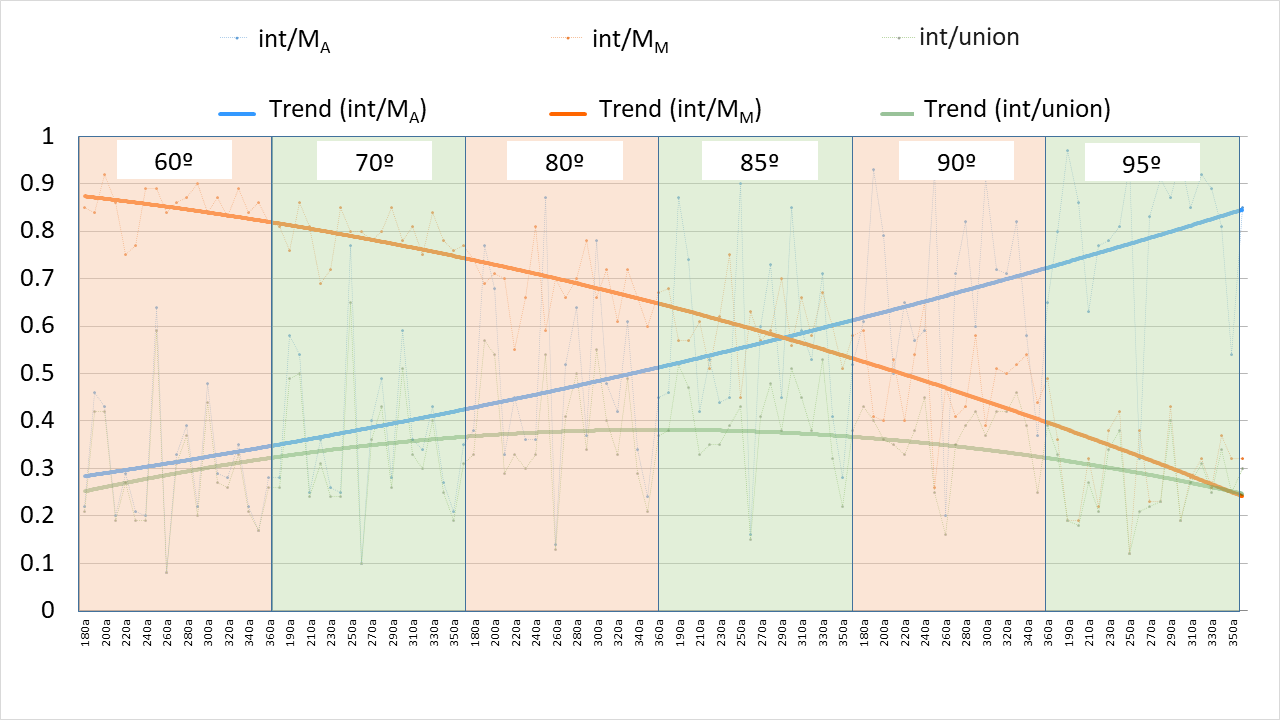
\includegraphics[width=\textwidth]{Imagenes/grafico.png}
         \hfill
         \caption{Curvas índice de calidad}
        \label{curvas_QI}
\end{figure}

%%%%%%%%%%%%%%%%%%%%%%%%%%%%%%%%%%%%%%%%%%%%%%
\begin{figure}
     \centering
     \begin{subfigure}[b]{0.3\textwidth}
         \centering
         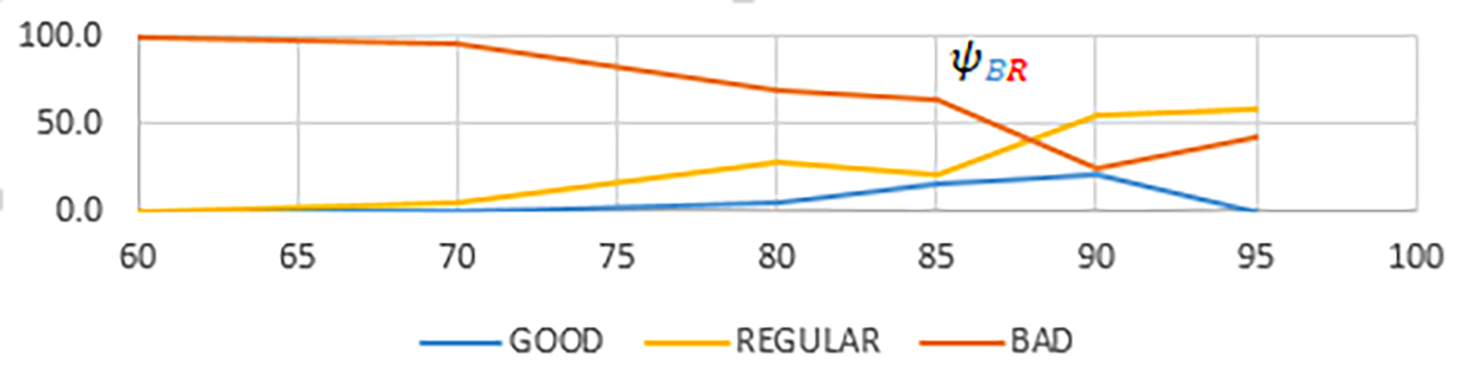
\includegraphics[width=\textwidth]{Imagenes/psiBR.png}
         \caption{\textpsi \textsubscript{BR}}
         \label{psiBR}
     \end{subfigure}
     \hfill
     \begin{subfigure}[b]{0.3\textwidth}
         \centering
         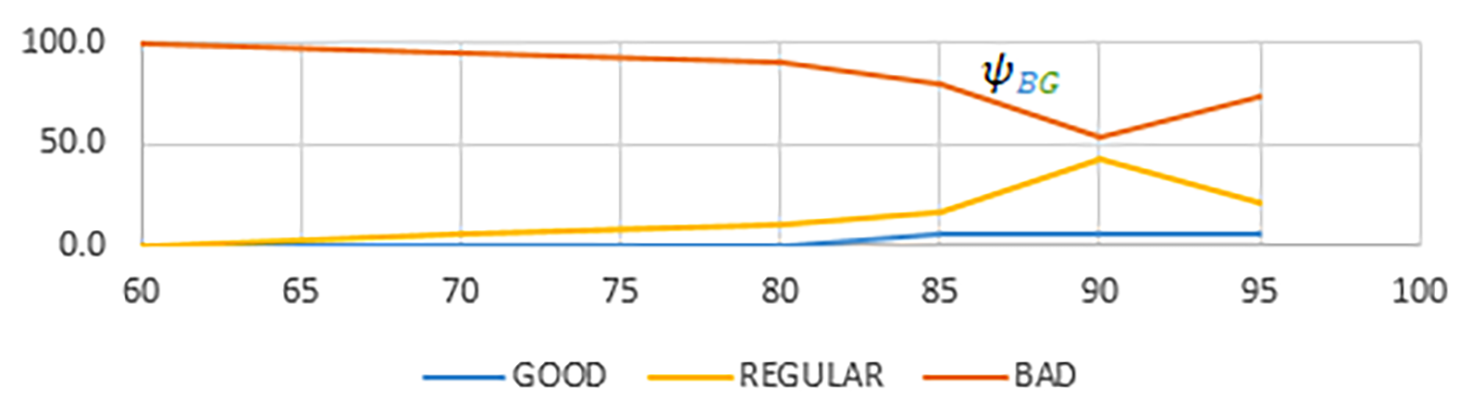
\includegraphics[width=\textwidth]{Imagenes/psiBG.png}
         \caption{\textpsi \textsubscript{BG}}
         \label{psiBG}
     \end{subfigure}
     \hfill
     \begin{subfigure}[b]{0.3\textwidth}
         \centering
         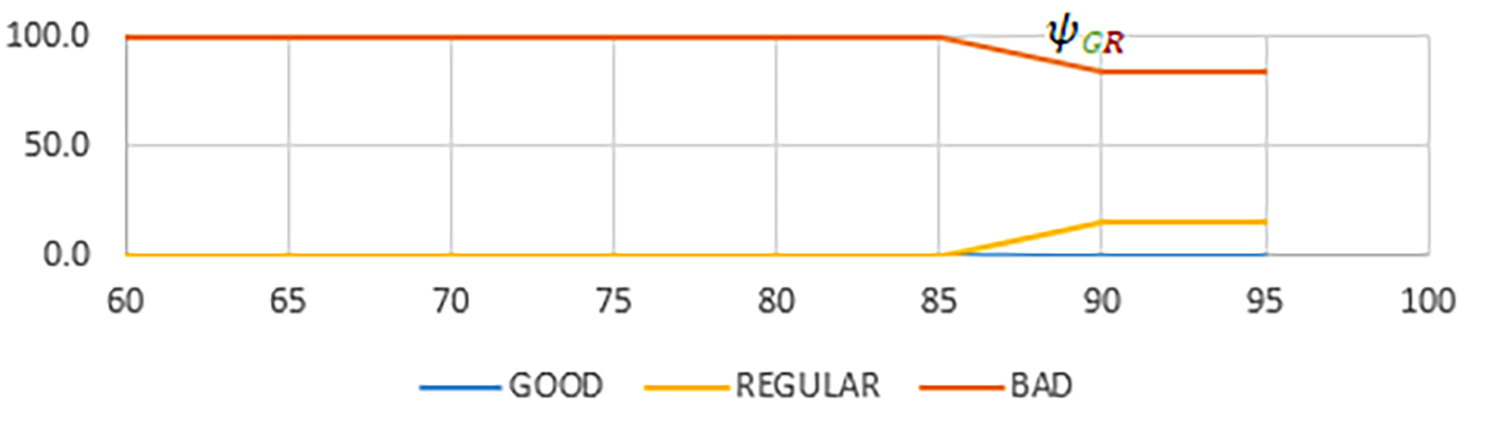
\includegraphics[width=\textwidth]{Imagenes/psiGR.png}
         \caption{\textpsi \textsubscript{GR}}
         \label{psiGR}
     \end{subfigure}
        \caption{Qualification of overlapping of both, manual and automatic masks by human experts}
        \label{humanscoring}
\end{figure}
\subsubsection{Conclusiones} \label{Conclusiones}

El procedimiento propuesto usando el índice invariante de color se puede aplicar para la detección de sombras en imágenes aéreas de áreas selváticas, usando recursos computacionales relativamente simples. Los resultados mostraron que el 85º percentil de la distribución de frecuencia del índice invariante de color obtenido por medio de la ecuación \ref{eq1} y la diferencia entre canales como el numerador, son parámetros aceptables para calcular el valor de umbral para la binarización y desde ahí obtener la máscara que corresponde a las áreas sombreadas.
En ambos casos, en que los numeradores son la diferencia entre azul y verde y azul y rojo, se presentaron los resultados mejores. Se encontró un método de comparación que permite evaluar el desempeño del algoritmo, en el que el índice de calidad QI se definió como el cociente entre la intersección resultante entre ambas máscaras, manual y automática, sobr ela unión resultante de ambas. De esta manera, si el índice se aproxima al valor 1 implica un mayor nivel de coincidencia entre ambas máscaras. Los resultados del algoritmo se comparan con la selección manual llevada a cabo por expertos, como puede apreciarse de las máscaras superpuestas sobre las imágenes. Si bien este método tiene algunas limitaciones, se puede aplicar sobre imágenes RGB, las que tienen algunos condicionantes en el momento de captura, y condiciones meteorológicas, como la presencia de nubes. Para asegurar la visibilidad de sombras en la imagen, la captura de las mismas debe hacerse en una franja horaria de 8 a.m. a 11 a.m. y de 2 p.m. a 5 p.m., dependiendo de la época del año y de la latitud. Otra limitación es la captura de imágenes con un cielo cubierto, ya que las sombras se presentan muy tenues. No obstanteeste método es una opción aceptable para automatizar la tarea de segmentación ed sombras en imágenes aéreas.

\subsection{C3-Filtros de texturas (probados con fantomas)}
Mediante el filtrado por textura puede implementarse una segmentación o clasificación en imágenes. Se hicieron varias pruebas con imágenes simuladas (cuadrados y rombos)
\subsection{C4-Mapas autoorganizados (clasificación no supervisada)}
\subsection{C5-IIC: Análisis de efecto de bandas utilizadas (sombras)}
Informe 1
Se realizaron pruebas del algoritmo sobre distintas imágenes que contienen sombra para ver su desempeño en la selección automática de sombras. Para todos los casos se aplicó para definir el umbral de binarización el correspondiente al percentil 85 de la distribución de frecuencias del índice invariante de color calculado por la ecuación \ref{invariante de color 1}:
 %%%%%%%%%%%%%%%%%%%%%%%%%%%%%%%%%%%%%% ECUACIÓN %%%%%%%%%%%%%%%%%%%%%%%%%%%%%%%%%%%%%%%%%%%%%%%%%%%%%%%%%
\\
\begin{equation}
	\psi=\frac{4}{\pi} arctan\left(\frac{B\textsubscript{1}-B\textsubscript{2}}{B\textsubscript{1}+B\textsubscript{2}}\right),\label{invariante de color 1}
\end{equation}
\\
%%%%%%%%%%%%%%%%%%%%%%%%%%%%%%%%%%%%%%%%%%%%%%%%%%%%%%%%%%%%%%%%%%%%%%%%%%%%%%%%%%%%%%%%%%%%%%%%%%%%%%%%%
La imagen de la izquierda se procesó con la combinación de las bandas azul y verde, la de la derecha con la combinación azul y rojo.
Se observa que hay mucha similitud en las áreas marcadas, no obstante los diferentes valores de binarización, obtenidos por criterio del 85to percentil de la distribución de frecuencias de los valores de índice invariante de color hallados para cada combinación de bandas.
\\
\\
Informe 2
Aplicando el algoritmo sobre una imagen seleccionada que contiene sombras, usando la ecuación \ref{invariante de color 2} en la combinación de bandas verde y roja y sin utilizar el criterio de percentil para definir el umbral de binarización:
%%%%%%%%%%%%%%%%%%%%%%%%%%%%%%%%%%%%%% ECUACIÓN %%%%%%%%%%%%%%%%%%%%%%%%%%%%%%%%%%%%%%%%%%%%%%%%%%%%%%%%%
\\
\begin{equation}
	\psi=\frac{4}{\pi} arctan\left(\frac{B\textsubscript{1}-B\textsubscript{2}}{B\textsubscript{1}+B\textsubscript{2}}\right),\label{invariante de color2}
\end{equation}
\\
%%%%%%%%%%%%%%%%%%%%%%%%%%%%%%%%%%%%%%%%%%%%%%%%%%%%%%%%%%%%%%%%%%%%%%%%%%%%%%%%%%%%%%%%%%%%%%%%%%%%%%%%%
Observando la imagen con la máscara superpuesta en color azul se nota una marcación altamente coincidente con la que corresponde al área sombreada. Además, mediante el gráfico de histograma de frecuencias del índice invariante de color es posible advertir el valle entre dos picos situado en torno al valor 0,2 el cual fue usado como umbral de binarización.
\\
\\
Informe 3

Tal como surge de la ecuación 1, las posibilidades de combinar dos entre tres bandas de color resultan en seis diferentes índices invariantes de color para una imagen dada. Lo que resulta notorio es que a priori no se sabe cuál de esas seis resulta la más adecuada para constituir la máscara de selección automática de sombras. 

